\documentclass[a4paper,12pt,twoside]{memoir}

% Castellano
\usepackage[spanish,es-tabla]{babel}
\selectlanguage{spanish}
\usepackage[utf8]{inputenc}
\usepackage[T1]{fontenc}
\usepackage{lmodern} % Scalable font
\usepackage{microtype}
\usepackage{placeins}

\RequirePackage{booktabs}
\RequirePackage[table]{xcolor}
\RequirePackage{xtab}
\RequirePackage{multirow}

% Links
\PassOptionsToPackage{hyphens}{url}\usepackage[colorlinks]{hyperref}
\hypersetup{
	allcolors = {red}
}

% Ecuaciones
\usepackage{amsmath}

% Rutas de fichero / paquete
\newcommand{\ruta}[1]{{\sffamily #1}}

% Párrafos
\nonzeroparskip

% Huérfanas y viudas
\widowpenalty100000
\clubpenalty100000

\let\tmp\oddsidemargin
\let\oddsidemargin\evensidemargin
\let\evensidemargin\tmp
\reversemarginpar

% Imágenes

% Comando para insertar una imagen en un lugar concreto.
% Los parámetros son:
% 1 --> Ruta absoluta/relativa de la figura
% 2 --> Texto a pie de figura
% 3 --> Tamaño en tanto por uno relativo al ancho de página
\usepackage{graphicx}

\newcommand{\imagen}[3]{
	\begin{figure}[!h]
		\centering
		\includegraphics[width=#3\textwidth]{#1}
		\caption{#2}\label{fig:#1}
	\end{figure}
	\FloatBarrier
}







\graphicspath{ {./img/} }

% Capítulos
\chapterstyle{bianchi}
\newcommand{\capitulo}[2]{
	\setcounter{chapter}{#1}
	\setcounter{section}{0}
	\setcounter{figure}{0}
	\setcounter{table}{0}
	\chapter*{#2}
	\addcontentsline{toc}{chapter}{#2}
	\markboth{#2}{#2}
}

% Apéndices
\renewcommand{\appendixname}{Apéndice}
\renewcommand*\cftappendixname{\appendixname}

\newcommand{\apendice}[1]{
	%\renewcommand{\thechapter}{A}
	\chapter{#1}
}

\renewcommand*\cftappendixname{\appendixname\ }

% Formato de portada

\makeatletter
\usepackage{xcolor}
\newcommand{\tutor}[1]{\def\@tutor{#1}}
\newcommand{\tutorb}[1]{\def\@tutorb{#1}}

\newcommand{\course}[1]{\def\@course{#1}}
\definecolor{cpardoBox}{HTML}{E6E6FF}
\def\maketitle{
  \null
  \thispagestyle{empty}
  % Cabecera ----------------
\begin{center}
  \noindent
\includegraphics[width=\textwidth]{cabeceraSalud}\vspace{1.5cm}%
\end{center}
  
  % Título proyecto y escudo salud ----------------
  \begin{center}
    \begin{minipage}[c][1.5cm][c]{.20\textwidth}
        
\includegraphics[width=\textwidth]{escudoSalud.pdf}
    \end{minipage}
  \end{center}
  
  \begin{center}
    \colorbox{cpardoBox}{%
        \begin{minipage}{.8\textwidth}
          \vspace{.5cm}\Large
          \begin{center}
          \textbf{TFG del Grado en Ingeniería de la Salud}\vspace{.6cm}\\
          \textbf{\LARGE\@title{}}
          \end{center}
          \vspace{.2cm}
        \end{minipage}
    }%
  \end{center}
  
    % Datos de alumno, curso y tutores ------------------
  \begin{center}%
  {%
    \noindent\LARGE
    Presentado por \@author{}\\ 
    en Universidad de Burgos\\
    \vspace{0.5cm}
    \noindent\Large
    \@date{}\\
    \vspace{0.5cm}
    Tutor: \@tutor{}\\ % comenta el que no corresponda
    %Tutores: \@tutor{} -- \@tutorb{}\\
  }%
  \end{center}%
  \null
  \cleardoublepage
  }
\makeatother

\newcommand{\nombre}{Mario de la Arena del Hoyo}
\newcommand{\nombreTutor}{Pedro Luis Sánchez Ortega} 
\newcommand{\nombreTutorb}{Tutor 2} 
\newcommand{\dni}{71482626Y} 

% Datos de portada
\title{Uso y aplicaciones de dispositivos comerciales de BCI en los entornos de salud}
\author{\nombre}
\tutor{\nombreTutor}
\tutorb{\nombreTutorb}
\date{\today}


\begin{document}

\maketitle


\newpage\null\thispagestyle{empty}\newpage

%%%%%%%%%%%%%%%%%%%%%%%%%%%%%%%%%%%%%%%%%%%%%%%%%%%%%%%%%%%%%%%%%%%%%%%%%%%%%%%%%%%%%%%%
\thispagestyle{empty}


\noindent
\includegraphics[width=\textwidth]{cabeceraSalud}\vspace{1cm}

\noindent D. \nombreTutor, profesor del departamento de departamento, área de área.

\noindent Expone:

\noindent Que el alumno D. \nombre, con DNI \dni, ha realizado el Trabajo final de Grado en Ingeniería de la Salud titulado título del trabajo. 

\noindent Y que dicho trabajo ha sido realizado por el alumno bajo la dirección del que suscribe, en virtud de lo cual se autoriza su presentación y defensa.

\begin{center} %\large
En Burgos, {\large \today}
\end{center}

\vfill\vfill\vfill

% Author and supervisor
%\begin{minipage}{0.45\textwidth}
%\begin{flushleft} %\large
%Vº. Bº. del Tutor:\\[2cm]
%D. \nombreTutor
%\end{flushleft}
%\end{minipage}
%\hfill
%\begin{minipage}{0.45\textwidth}
%\begin{flushleft} %\large
%Vº. Bº. del Tutor:\\[2cm]
%D. \nombreTutorb
%\end{flushleft}
%\end{minipage}
%\hfill

%\vfill

% para casos con solo un tutor comentar lo anterior
% y descomentar lo siguiente
Vº. Bº. del Tutor:\\[2cm]
D. \nombreTutor


\newpage\null\thispagestyle{empty}\newpage




\frontmatter

% Abstract en castellano
\renewcommand*\abstractname{Resumen}
\begin{abstract}
En este primer apartado se hace una \textbf{breve} presentación del tema que se aborda en el proyecto.
\end{abstract}

\renewcommand*\abstractname{Descriptores}
\begin{abstract}
Palabras separadas por comas que identifiquen el contenido del proyecto Ej: servidor web, buscador de vuelos, android \ldots
\end{abstract}

\clearpage

% Abstract en inglés
\renewcommand*\abstractname{Abstract}
\begin{abstract}
A \textbf{brief} presentation of the topic addressed in the project.
\end{abstract}

\renewcommand*\abstractname{Keywords}
\begin{abstract}
keywords separated by commas.
\end{abstract}

\clearpage

% Indices
\tableofcontents

\clearpage

\listoffigures

\clearpage

\listoftables
\clearpage


\mainmatter
\capitulo{1}{Introducción}

Este proyecto se centra en el estudio y uso del dispositivo Emotiv MN8, un dispositivo de electroencefalografía (EEG) innovador. El objetivo principal es realizar una serie de pruebas para comprender a fondo su funcionamiento y los datos que adquiere y analiza.

En la primera fase del proyecto, se realizarán pruebas con el dispositivo MN8 y las aplicaciones asociadas, Emotiv y Contour. Estas pruebas permiten familiarizarse con las capacidades del dispositivo y los métodos de recopilación y análisis de datos.

Una vez comprendido el funcionamiento del dispositivo y las aplicaciones, el siguiente paso es diseñar y realizar una serie de experimentos que impliquen el uso del EEG Emotiv MN8. Estos experimentos estarán diseñados para crear situaciones controladas, lo que permitirá recoger y analizar los resultados obtenidos.

Finalmente, el objetivo es evaluar la validez del dispositivo MN8 para su uso en el ámbito médico. Se espera que este proyecto proporcione una valiosa contribución a la comprensión de cómo se pueden utilizar los dispositivos EEG en la práctica médica y cómo los datos recogidos pueden ser utilizados para informar y mejorar las prácticas y estrategias.

Este proyecto representa una oportunidad para explorar el potencial de la tecnología EEG y su aplicación en el ámbito médico.

\capitulo{2}{Objetivos}

Este apartado explica de forma precisa y concisa cuales son los objetivos que se persiguen con la realización del proyecto. Se puede distinguir entre:
\subsubsection{Objetivos Generales}
\begin{enumerate}
    \item Uso y aplicaciones de dispositivos comerciales de BCI en los entornos de salud.
\end{enumerate}

\subsubsection{Objetivos Específicos}
\begin{enumerate}
    \item Comprender el funcionamiento del dispositivo Emotiv MN8, lo que implica realizar una serie de pruebas para entender cómo funciona el dispositivo y cómo adquiere y analiza los datos.
    \item Familiarizarse con las capacidades del dispositivo y los métodos de recopilación y análisis de datos mediante pruebas con el dispositivo MN8 y las aplicaciones asociadas, Emotiv y Contour.
    \item Diseñar y realizar una serie de experimentos en el entorno de PsychoPy \cite{psychopyOverview}\footnote{Página web de PsychoPy con la información general de la aplicación \cite{psychopyOverview}.} utilizando el EEG Emotiv MN8 para crear situaciones controladas que permitan recoger y analizar los resultados obtenidos.
    \item Evaluar la validez del dispositivo MN8 para su uso en el ámbito sanitario.
    \item Contribuir a la comprensión de cómo se pueden utilizar los dispositivos EEG portables en la práctica sanitaria, lo que permitiría informar y mejorar las prácticas y estrategias médicas.
    \item Usar herramientas como GitHub \cite{GitHub}\footnote{Repositorio de GitHub con toda la documentación del TFG \cite{GitHub}.} para el seguimiento de los documentos del trabajo y la recopilación del código de los programas y documentos realizados en el proyecto.
    \item Emplear Overleaf \cite{overleaf}\footnote{Enlace de la herramienta Overleaf \cite{overleaf}.} como editor LaTex para la creación de los documentos entregables.
    \item  Analizar costes y viabilidad legal del proyecto propuesto.
    \item Realizar un trabajo reproducible en el futuro para que otras personas puedan realizar los prototipos gracias a los datos y conocimientos desarrollados en el proyecto.
\end{enumerate}

\capitulo{3}{Conceptos teóricos}

\section{Conceptos teóricos básicos}

Para comprender este proyecto, es necesario familiarizarse con los siguientes conceptos teóricos básicos:
\begin{itemize}
    \item \textbf{Electroencefalografía}: Es una técnica de registro de la actividad eléctrica del cerebro. Se utiliza principalmente en medicina, psicología y neurociencia para estudiar el funcionamiento del cerebro.
    \item \textbf{Dispositivo Emotiv MN8}: Es un dispositivo de EEG portátil e inalámbrico que permite la recopilación de datos de EEG en tiempo real. Este dispositivo es capaz de registrar la actividad eléctrica del cerebro y transmitirla a una computadora o dispositivo móvil para su análisis. Se puede ver cómo es en la imagen \ref{fig: EmotivMN8} y también en que partes se colocan en la imagen \ref{fig: PosicionSensoresMN8}
    \begin{figure}[h]
    \centering
    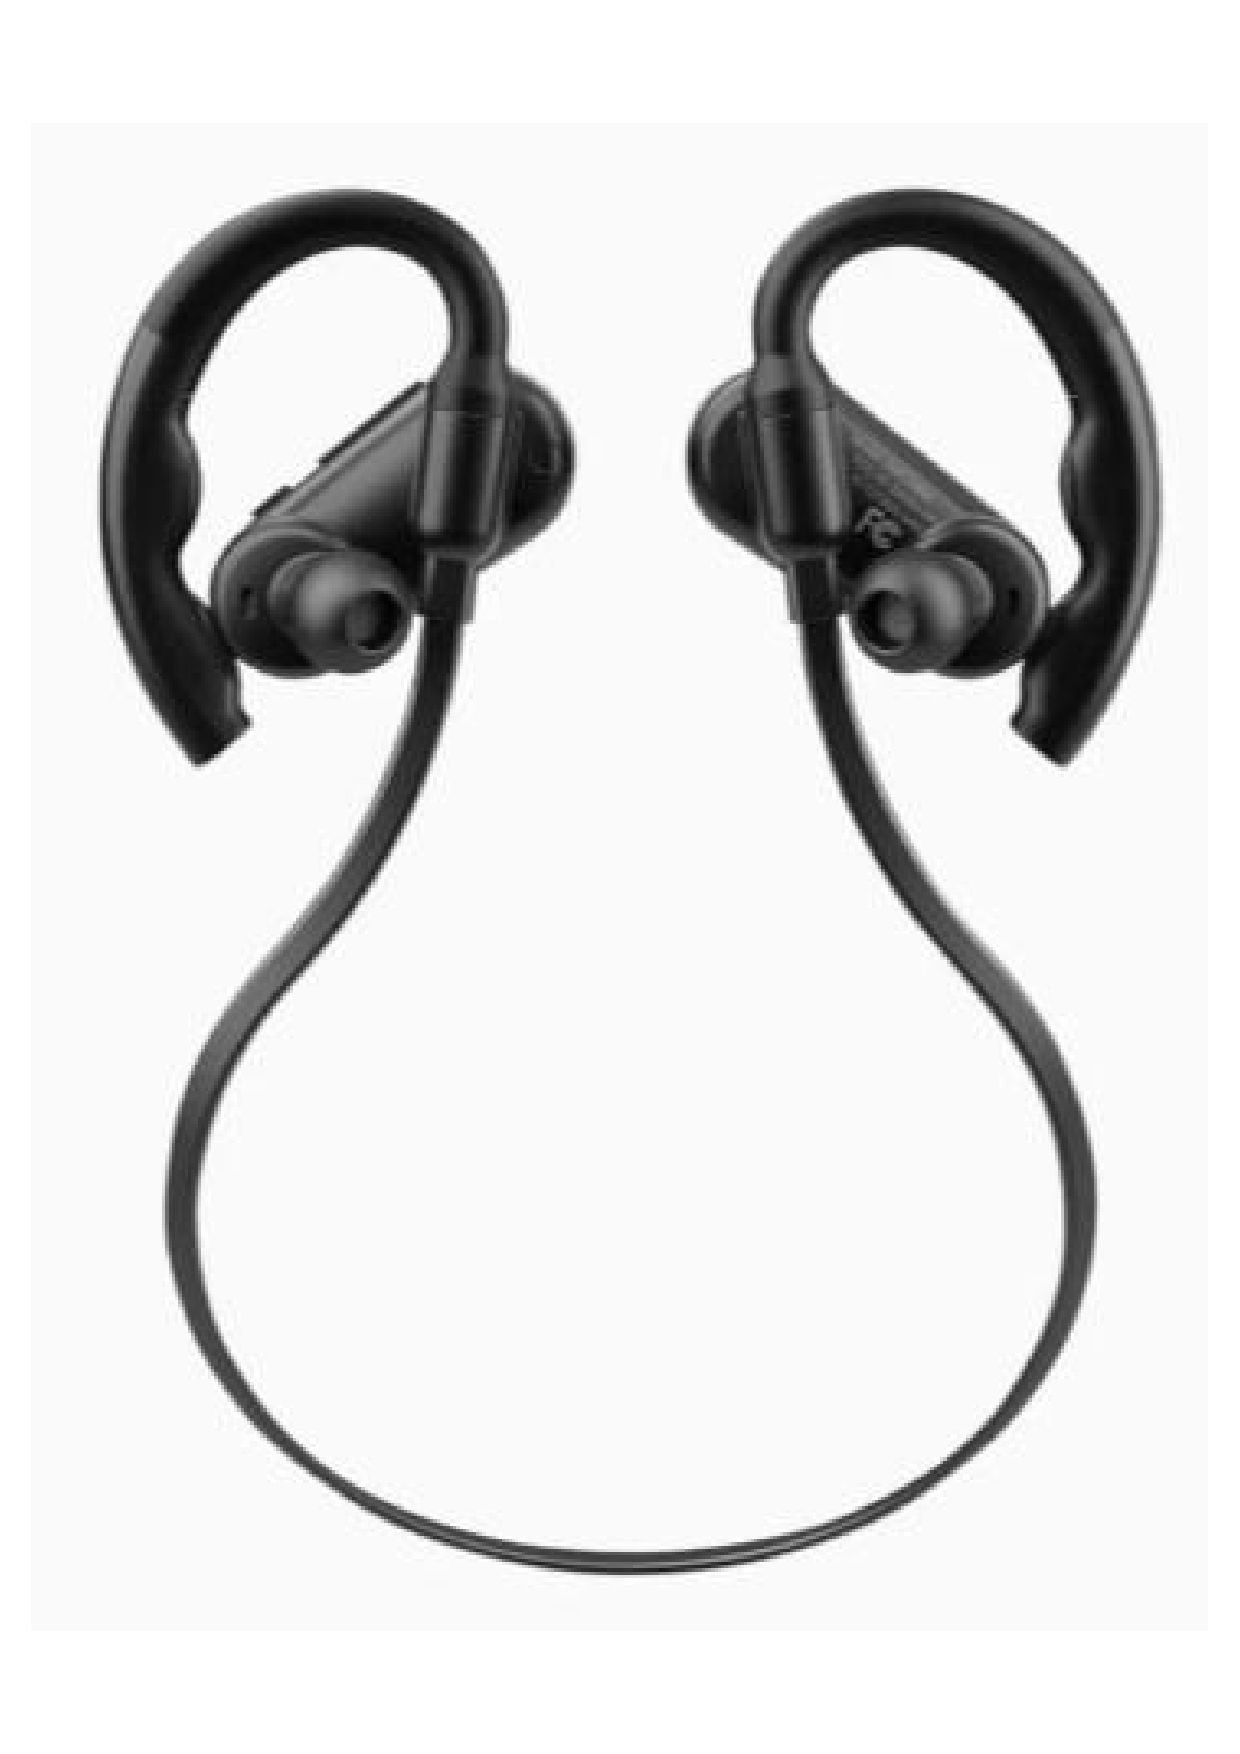
\includegraphics[width=0.3\textwidth]{img/DispositivoEmotivMN8.pdf}
    \caption{Dispositivo Emotiv MN8.}
    \label{fig: EmotivMN8}
    \end{figure}
    
    \begin{figure}[h]
    \centering
    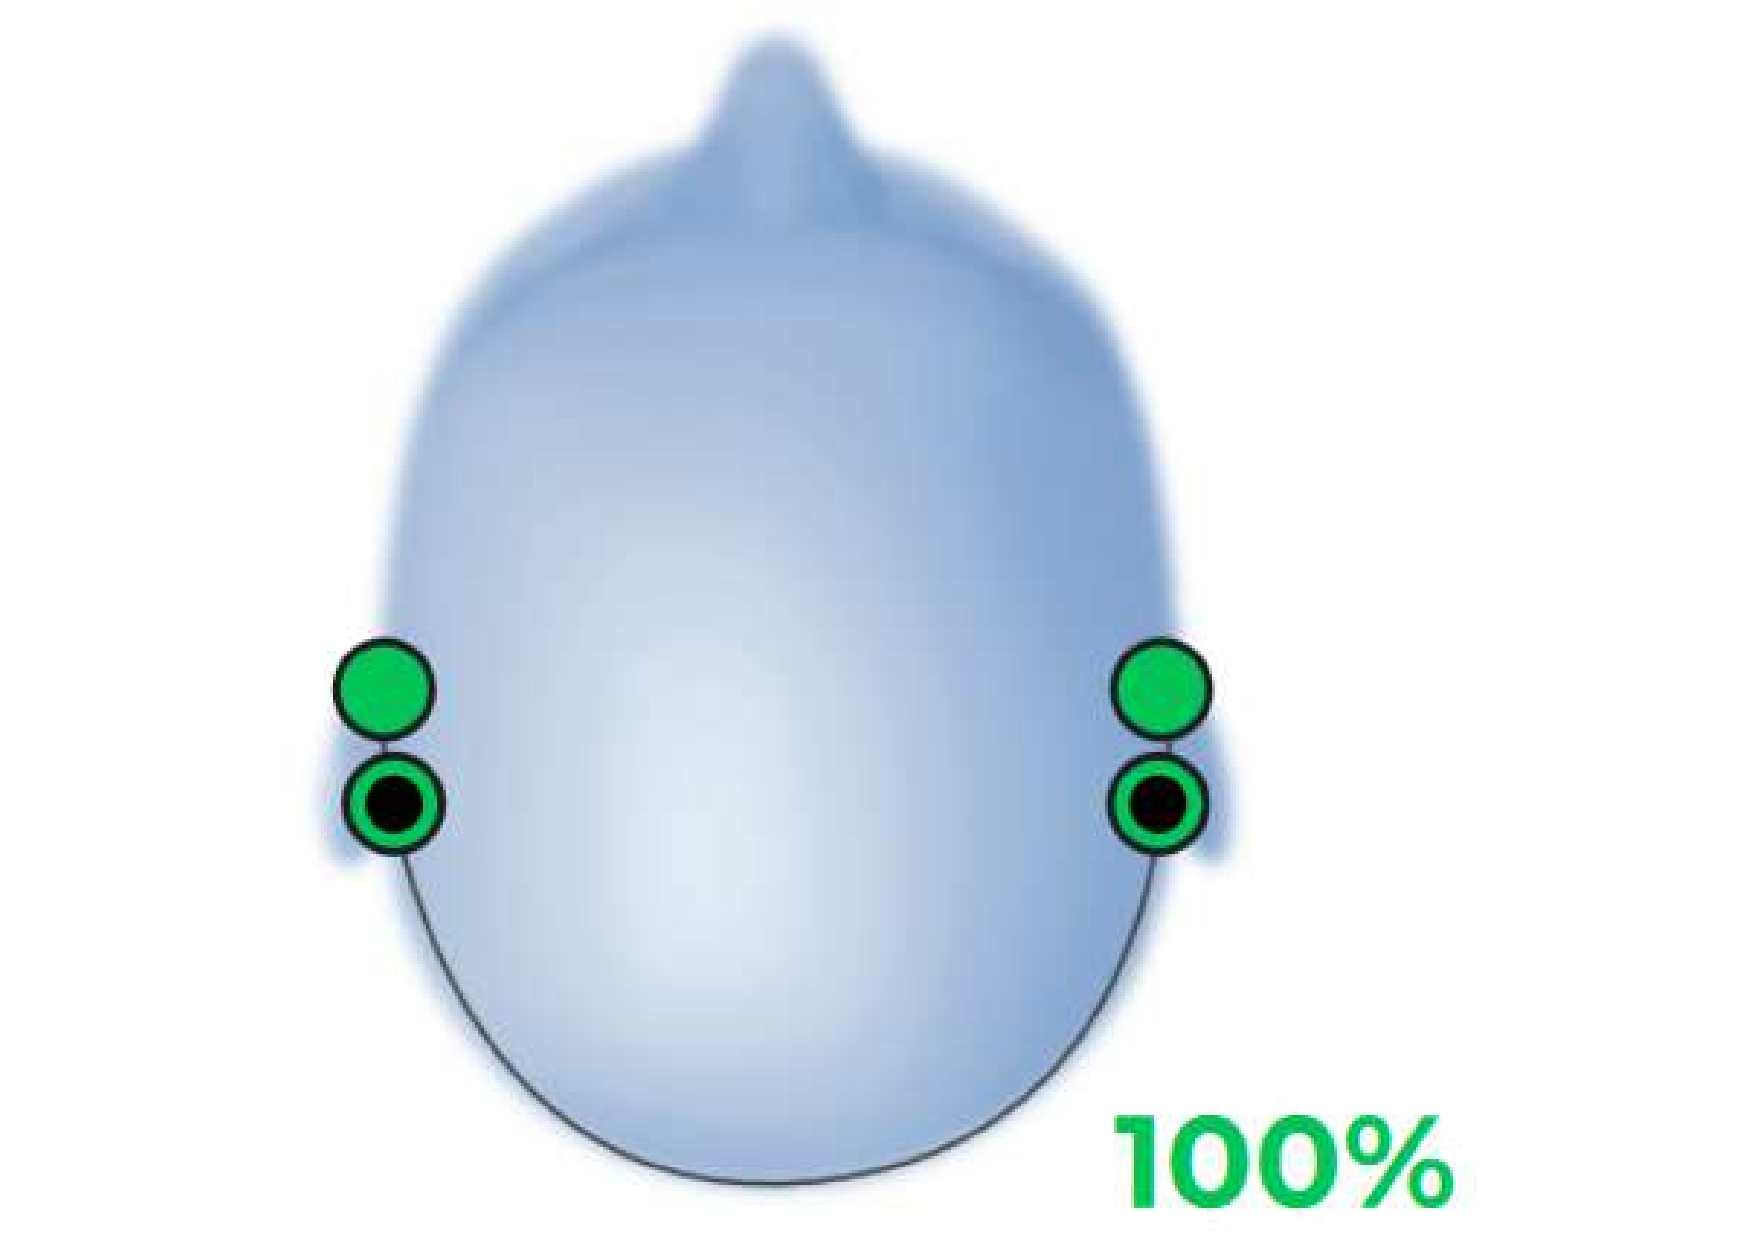
\includegraphics[width=0.5\textwidth]{img/PosicionSensoresMN8.pdf}
    \caption{Posición sensores MN8.}
    \label{fig: PosicionSensoresMN8}
    \end{figure}
    \item \textbf{Aplicaciones Emotiv y Contour}: Son aplicaciones de \textit{software} que se utilizan junto con el dispositivo Emotiv MN8 para recoger y analizar los datos de EEG. Estas aplicaciones permiten visualizar los datos de EEG en tiempo real y realizar análisis detallados de los mismos.
    \item \textbf{GitHub}: Es una plataforma en línea que facilita a las personas la posibilidad de trabajar en proyectos de programación de manera colaborativa. Permite a los usuarios guardar versiones de su código, lo que significa que pueden guardar diferentes versiones de su trabajo y volver a una versión anterior si es necesario. También proporciona un lugar para compartir proyectos de código abierto, lo que significa que cualquier persona puede ver, usar o contribuir a los proyectos alojados allí. Por lo tanto, es una herramienta útil para el desarrollo de software, ya sea de manera individual o en equipo. 
    \item \textbf{Diseño experimental}: Es el proceso de planificación de un experimento para asegurar que los datos recogidos sean válidos y confiables. En este proyecto, se diseñarán experimentos para crear situaciones controladas que permitan recoger y analizar los datos de EEG.
    \item \textbf{PsychoPy}: Es un \textit{software} gratuito que permite a los investigadores crear experimentos de neurociencia y psicología. Ofrece una interfaz sencilla para la presentación de estímulos y el control de experimentos, y puede ser utilizado tanto en ordenadores como en dispositivos móviles.
    \item \textbf{Análisis de datos}: Es el proceso de inspeccionar, limpiar y modelar los datos recogidos con el objetivo de descubrir información útil, informar conclusiones y apoyar la toma de decisiones.
    \item \textbf{Interfaz cerebro-computadora}: La interfaz cerebro-computadora, cuyas siglas son BCI y provienen de \textit{Brain–Computer Interfaces}, es un sistema que adquiere información neural, como datos de electrofisiología nerviosa o registros de ondas cerebrales, y la procesa e interpreta utilizando un ordenador \cite{InterfazBCI}\footnote{Artículo con información sobre qué es el BCI, así como su funcionamiento y sus aplicaciones \cite{InterfazBCI}.}. Estas interfaces permiten transformar el pensamiento en acciones reales en el entorno. Se aplican en diversas áreas, como la medicina (para el control de prótesis o rehabilitación), la investigación (con el estudio de la actividad cerebral) y la tecnología (por la interacción con dispositivos mediante el pensamiento).
    \item \textbf{EEG Headset}: Los \textit{EEG Headset} son dispositivos diseñados para medir y registrar la actividad eléctrica del cerebro. Estos dispositivos utilizan electrodos colocados en el cuero cabelludo para capturar los impulsos eléctricos generados por las células cerebrales o neuronas \cite{EEGHeadset}\footnote{Página web de Emotiv con toda la información general sobre los \textit{EEG Headsets} \cite{EEGHeadset}.}. Su uso se enfoca en comprender la actividad cerebral y su aplicación abarca desde la medicina hasta la investigación y la tecnología.
\end{itemize}
Estos conceptos proporcionan una base sólida para entender el proyecto y su objetivo de explorar el potencial de la tecnología EEG portable y su aplicación en el ámbito sanitario. Se espera que este proyecto proporcione una valiosa contribución a la comprensión de cómo se pueden utilizar los dispositivos EEG en la práctica médica y cómo los datos recogidos pueden ser utilizados para informar y mejorar las prácticas y estrategias.

\section{Estado del arte y trabajos relacionados.}
En esta sección, el conocimiento previo existente en el área específica del proyecto se analiza y se sintetiza en un resumen unificado. El propósito es situar el trabajo actual dentro del panorama científico y tecnológico, identificando las contribuciones previas, las limitaciones y las tendencias emergentes.
Por lo tanto, esta revisión abarca publicaciones científicas reales, patentes, proyectos previos y desarrollos relevantes.

\subsection{Aplicación de dispositivo de \textit{Interface neural} en Ingeniería de la Salud}
Para la realización de este proyecto, se ha tenido en cuenta el trabajo de fin de grado de Elena Pérez Barco, el cual es confidencial, por lo que no será referenciado para mantener la privacidad y derechos de autor, ya que el jurado tiene acceso a este trabajo.

Este trabajo se centra en una investigación comparativa de dispositivos EEG portátiles, analizando sus características técnicas, ventajas y desventajas, centrándose principalmente en el Emotiv Insight 2.0, un dispositivo EEG portátil ampliamente utilizado en investigaciones. Finalmente, se investigaron las posibles aplicaciones de estos dispositivos EEG portátiles en el ámbito de la salud.


\subsection{Dispositivos g.tec}
g.tec es una empresa que se encarga de desarrollar BCI y neurotecnologías de alto rendimiento, puediendo emplear técnicas invasivas y no invasivas en función del objetivo de las grabaciones \cite{g.tec}\footnote{Página web oficial de g.tec con información general de la empresa y sus productos \cite{g.tec}.}.

Uno de sus productos destacados es el g.Nautilus PRO, el cual se puede ver en la imagen \ref{fig: g.Nautilus}. Se trata de un auricular EEG portátil certificado por la CE (Conformidad Europea) y aprobado por la FDA (Administración de Alimentos y Medicamentos de los Estados Unidos) para registrar la actividad cerebral en entornos médicos y clínicos. Sus características más relevantes son \cite{g.Nautilus}\footnote{Sección del dispositivo g.Nautilus dentro de la página web oficial de g.tec \cite{g.Nautilus}.}:
\begin{itemize}
    \item Electrodos EEG: Disponible con 8, 16 o 32 electrodos EEG secos o húmedos prefijados para realizar un montaje más rápido.
    \item Versatilidad: Permite grabaciones secas y húmedas con un solo electrodo.
    \item Aplicaciones clínicas: Útil para monitoreo cerebral en entornos médicos y estudios de investigación.
    \item Electrodos activos: Hay 2 tipos de electrodos, electrodos activos secos 'g.SAHARA' o electrodos activos húmedos 'g.LADYbird'. Los electrodos 'g.SAHARA HYBRID' se caracterizan por:
    \begin{itemize}
        \item Tecnología patentada: Es el primer sistema de electrodos secos que funciona en todos los sitios cerebrales (frontal, central, occipital, temporal y parietal).
        \item Electrodo híbrido: Permite grabaciones secas y húmedas con un solo electrodo.
    \end{itemize}
\end{itemize}

\begin{figure}[H]
    \centering
    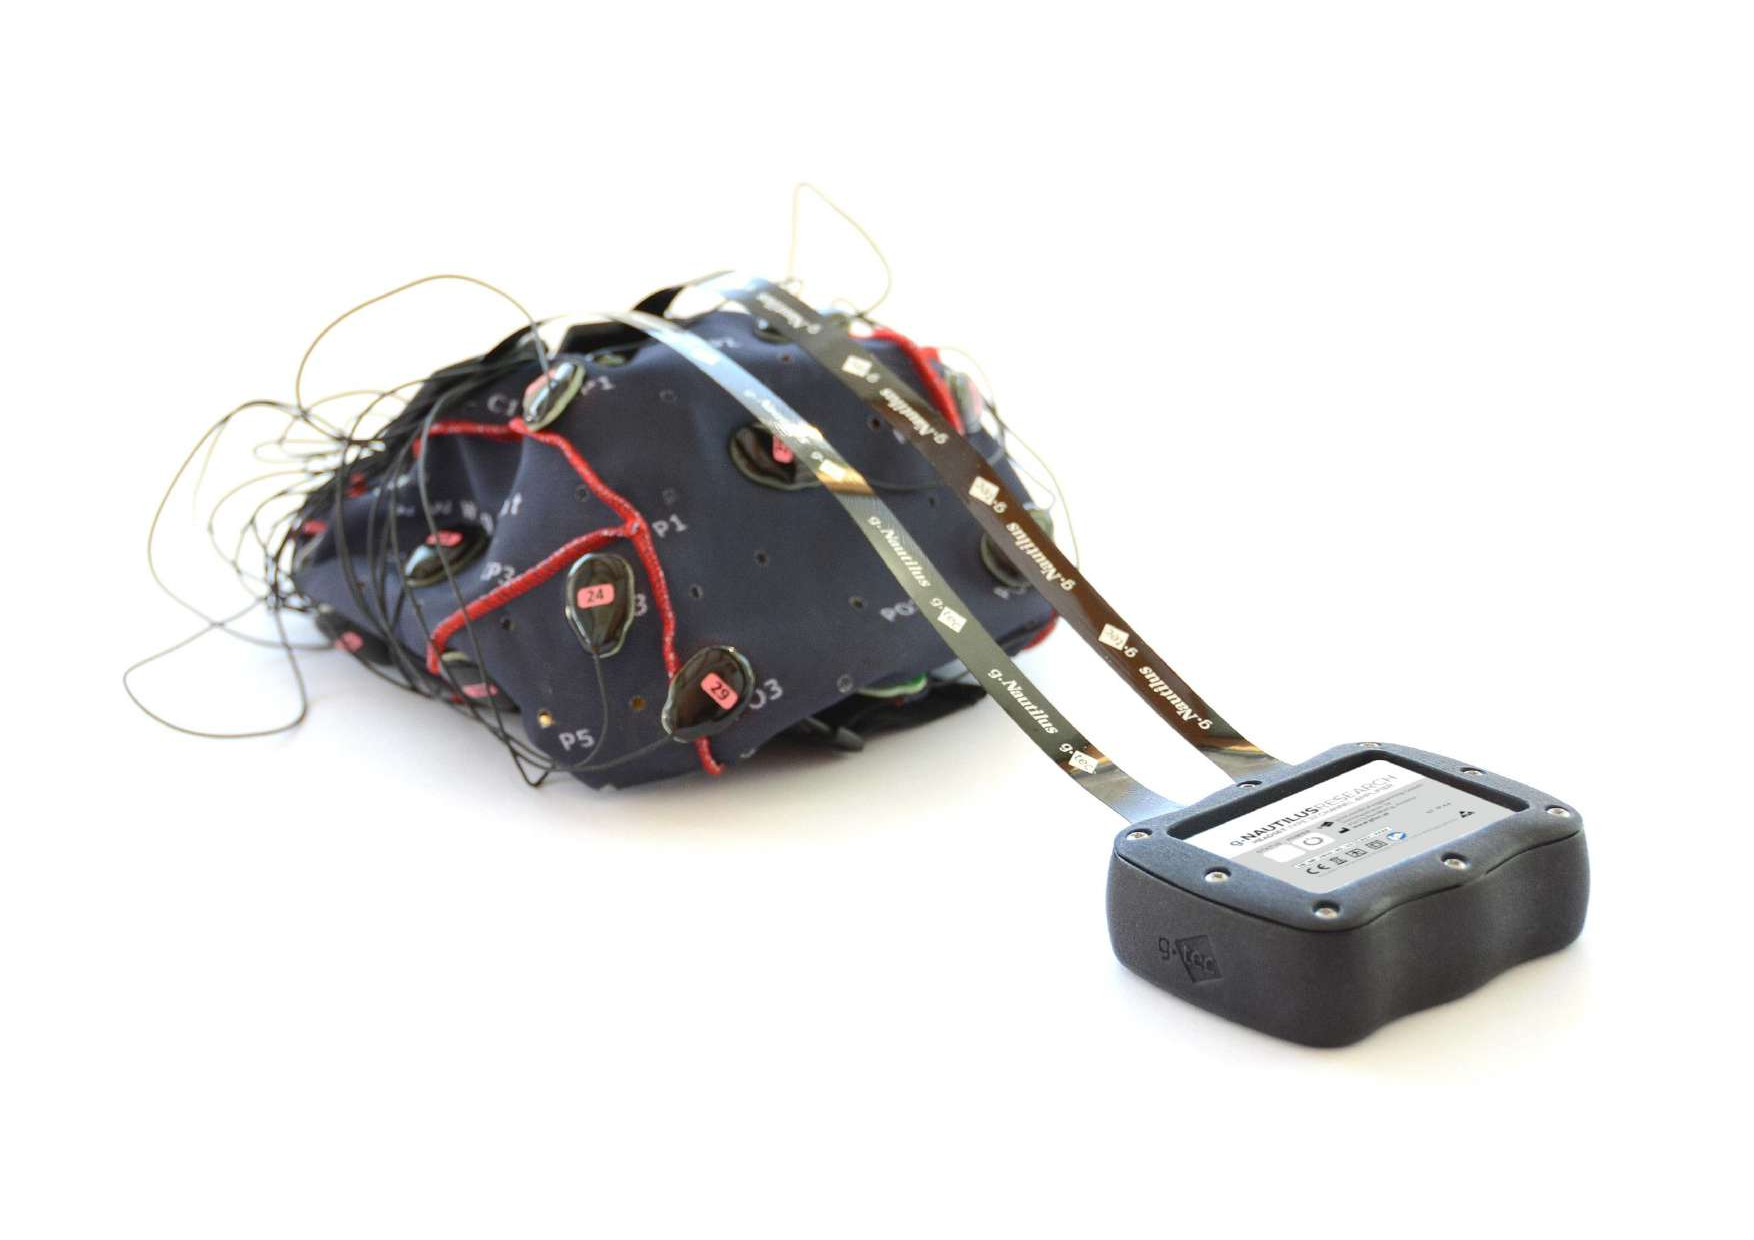
\includegraphics[width=0.4\textwidth]{img/g.Nautilus.pdf}
    \caption{Dispositivo g.Nautilus.}
    \label{fig: g.Nautilus}
\end{figure}

Por lo tanto, el 'g.Nautilus PRO' es una herramienta valiosa para la monitorización cerebral, la investigación y el diagnóstico en entornos médicos y clínicos. Su diseño modular y su capacidad de adaptación lo convierten en una opción versátil para profesionales de la salud y científicos interesados en la actividad cerebral.

\subsection{Uso de BCI para controlar máquinas.}
En 2024, un científico español y su equipo han desarrollado una BCI \cite{ArticuloControlBCI}\footnote{Página del árticulo del desarrollo de una BCI para controlar dispositivos con la mente \cite{ArticuloControlBCI}.}. La posibilidad de controlar dispositivos tecnológicos mediante el pensamiento, ha sido objeto de investigaciones en todo el mundo. Las BCI han demostrado eficacia en el control de exoesqueletos y la traducción de actividad neuronal en palabras. Sin embargo, muchas aproximaciones requieren implantes invasivos.

El investigador español José del R. Millán se ha enfocado en interfaces no invasivas y universales, permitiendo a cualquiera aprender a usarlas. Su equipo recientemente logró que personas sanas controlaran con precisión un coche en un videojuego de carreras utilizando solo la mente, sin mandos físicos. El objetivo de este proyecto es trasladar la BCI al ámbito clínico y mejorar la accesibilidad para personas con discapacidad. Este avance podría allanar el camino para entrenar a pacientes en el manejo de dispositivos de asistencia y neurorrehabilitación controlados por BCI.

El laboratorio del investigador español José del R. Millán se ha dedicado durante más de dos décadas al desarrollo de BCI con el objetivo de ayudar a personas con discapacidades motoras. Estas interfaces permiten a los usuarios controlar dispositivos mediante señales cerebrales, pero su calibración previa suele ser prolongada y específica para cada individuo. La solución propuesta por el equipo de Millán permite una autocalibración más rápida al entender las necesidades y señales cerebrales de cada sujeto. Esto acorta los plazos y facilita el uso del dispositivo sin adaptación previa.

La interfaz no es invasiva y se basa en un gorro rojo con electrodos conectado a un ordenador. Los electrodos captan las señales eléctricas del cerebro, que luego son interpretadas por un descodificador. Los usuarios han logrado controlar un coche en un videojuego,como se muestra en la imagen \ref{fig: ExperimentoBCI}, y un programa de equilibrio de una barra digital, demostrando el éxito de este enfoque en la mejora de la plasticidad neuronal. Este avance podría transformar la vida de personas con discapacidad motora al proporcionarles una forma más eficiente y rápida de interactuar con la tecnología.

\begin{figure}[H]
    \centering
    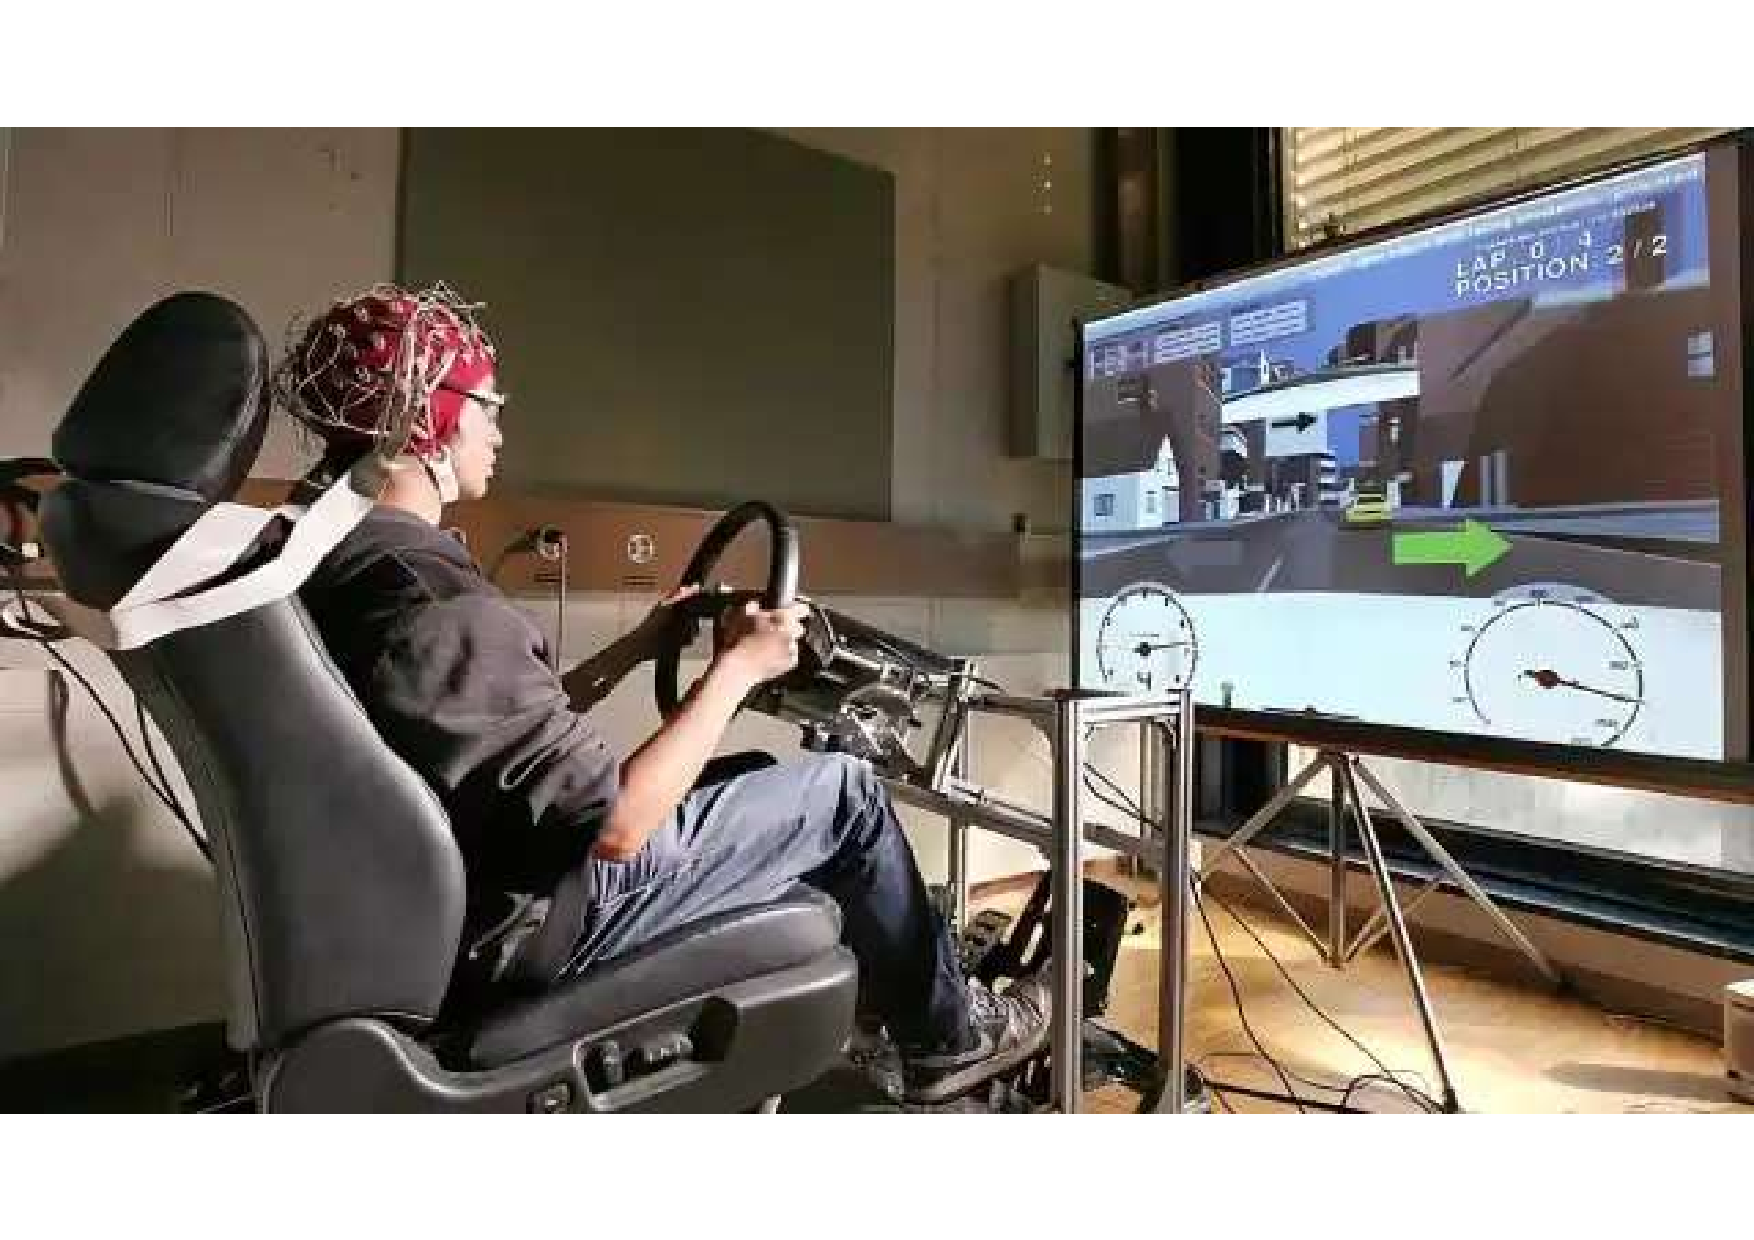
\includegraphics[width=0.6\textwidth]{img/ExperimentoBCI.pdf}
    \caption{Experimento realizado para avanzar en BCI.}
    \label{fig: ExperimentoBCI}
\end{figure}

 El siguiente paso programado por Millán es probar este método con personas que sí sufren algún tipo de discapacidad motora, La posibilidad de producir y distribuir comercialmente un dispositivo de estas características a gran escala aún queda muy lejos, pero esta investigación implica un descubrimiento fundacional, que sienta las bases de futuras innovaciones.

 \subsection{Síntesis del habla y expresiones faciales a partir de señales cerebrales}

 El síndrome de enclaustramiento es un estado neurológico en el que una persona está despierta y consciente, pero presenta cuadriplejía y parálisis de los nervios craneales inferiores. Esto significa que no puede moverse, hablar ni comunicarse, excepto a través de movimientos oculares codificados. Por lo general, se produce después de un accidente cerebrovascular que afecta la protuberancia, interrumpiendo y dañando los centros que controlan la mirada horizontal \cite{SindromeEnclaustramiento}\footnote{Página del NIH con información relativa al síndrome de enclaustramiento \cite{SindromeEnclaustramiento}.}.
 
 Ann Johnson, quien sufrió un derrame cerebral hace casi dos décadas, quedó paralizada y sin capacidad para hablar debido a este síndrome. Sin embargo, con un nuevo implante cerebral basado en inteligencia artificial, ha logrado sintetizar el habla y las expresiones faciales a partir de señales cerebrales, convirtiéndose en la primera paciente en utilizar con éxito esta tecnología innovadora. Los investigadores implantaron electrodos en su cerebro y personalizaron la tecnología para interpretar sus señales cerebrales. Aunque sus músculos no se mueven, su cerebro envía señales que los electrodos descodifican, permitiendo la síntesis del habla y las expresiones faciales mediante un avatar por ordenador.

Antes de este avance, Johnson podía comunicarse a unas 14 palabras por minuto utilizando un antiguo método de mecanografía que respondía a pequeños movimientos de su cabeza. Sin embargo, gracias a la inteligencia artificial, su avatar digital ahora habla a casi 80 palabras por minuto con el nuevo implante. El objetivo de esta tecnología es restablecer una forma de comunicación plena y corporal, que es la manera más natural de interactuar con los demás.

Aunque existen controversias y problemas éticos en el campo de la neurotecnología, avances como este ofrecen posibilidades reales para mejorar la vida humana, siendo un gran ejemplo de cómo la ciencia y la tecnología pueden transformar vidas de maneras inimaginables.

\capitulo{4}{Metodología}

\section{Descripción de los datos.}

Para la elaboración del proyecto, no se han utilizado datos predefinidos obtenidos de bases de datos existentes, sino que se han empleado datos de elaboración propia. Estos datos se diferencian entre los proporcionados por los usuarios y los proporcionados por el dispositivo.

Por un lado, los datos proporcionados por el usuario al crear su cuenta en la aplicación del dispositivo incluyen información personal como el nombre, apellidos, nombre de usuario, correo electrónico, edad y contraseña. Estos datos deben protegerse adecuadamente según las leyes españolas.

Por otro lado, los datos recopilados durante la monitorización del estrés y la concentración del usuario se obtienen mediante mediciones constantes realizadas a través del dispositivo MN8. Estas mediciones proporcionan información sobre el estrés, la concentración y la carga cognitiva del usuario. Cuando se detectan niveles elevados de estrés y bajos niveles de concentración, se emite una señal para que el usuario descanse o se relaje, permitiendo así que la actividad se desarrolle con niveles adecuados.

En el futuro, la recopilación de esta serie de datos de un gran número de personas podría facilitar la realización de estudios estadísticos sobre el estrés, la concentración y la carga cognitiva en diversas actividades y situaciones.

\section{Técnicas y herramientas.}
En este apartado se realiza una recopilación de técnicas y herramientas empleadas o valoradas en el desarrollo del proyecto.

\subsection{Lenguajes de programación empleados.}
En el grado se han enseñado varios lenguajes de programación, como Java, Python, LaTex, R o Markdown. Durante el desarrollo del proyecto se han empleado algunos de estos lenguajes de programación. Por ejemplo, para la creación de los documentos oficiales se ha usado el lenguaje LaTex, para la creación de las actividades en PsychoPy se ha empleado Python, mientras que para la presentación del repositorio de GitHub se ha utilizado Markdown.

\subsection{Entornos y aplicaciones empleadas.}
Para el desarrollo del proyecto, se han utilizado una serie de aplicaciones que han sido previamente empleadas en el grado, así como otras que no se han utilizado anteriormente.

\subsubsection{Overleaf}
Es un editor LaTeX colaborativo en línea, que se emplea para la creación, edición y publicación de documentos científicos. LaTeX es una herramienta que a partir del procesamiento de un documento de texto plano (compuesto por texto y comandos LaTeX) empleando el software de TeX engine, convierte los comandos LaTeX y el texto del documento en un archivo PDF profesional. Esta es la herramienta que se ha empleado para la realización de este documento \cite{overleaf}\footnote{Enlace de la herramienta Overleaf \cite{overleaf}.}.

\subsubsection{GitHub}
Plataforma gratuita en línea de código abierto cuyo objetivo principal es el desarrollo colaborativo de \textit{software}, para ello se basa en su sistema de control de versiones. GitHub fue construida empleando herramientas de código abierto cómo Ruby on Rails, Go, Primer, React o Kafka. Además, esta plataforma permite no solo la creación de proyectos públicos, sino que también proyectos privados que se guardan en la nube. Por otro lado, GitHub también tiene distintas herramientas que mejoran y dinamizan el desarrollo de los proyectos. Esta plataforma se ha empleado para llevar el seguimiento del proyecto y recopilar todos los documentos relacionados en un repositorio \cite{GitHub}\footnote{Página web oficial de la herramienta GitHub\cite{GitHub}.}.

\subsubsection{Stream}
Herramienta de Microsoft 365 diseñada para compartir videos a nivel empresarial. Ofrece características avanzadas como transcripción de audio, reconocimiento facial y transmisiones en vivo. Microsoft Stream se integra con otras aplicaciones de Microsoft, como Teams o SharePoint, facilitando el acceso y la difusión de contenido audiovisual. Su propósito principal es permitir a los usuarios crear, descubrir y compartir vídeos de manera segura dentro de la organización. Esta plataforma se ha empleado para realizar una transcripción de la actividad de 'Mindful Meditation' de Emotiv con el objetivo de traducirlo al castellano \cite{MicrosoftStream}\footnote{Página de Microsoft con toda la información acerca de Stream \cite{MicrosoftStream}.}.

\subsubsection{PsychoPy}
PsychoPy es un paquete de código abierto para ejecutar experimentos en Python. Combina las fortalezas gráficas de OpenGL con la sencillez de la sintaxis de Python para proporcionar a los científicos un paquete de presentación y control de estímulos gratuito y sencillo. Se utiliza en muchos laboratorios para la psicofísica, la neurociencia cognitiva y la psicología experimental.
Al ser de código abierto, puede descargarse y modificarse libremente, los cuales pueden ser compartidos con la comunidad para realizar la mayor cantidad de aportaciones posibles con el fin de mejorar la aplicación \cite{psychopyOverview}\footnote{Página principal de la web de PsychoPy con una pequeña introducción de la aplicación \cite{psychopyOverview}.}.

Esta aplicación presenta dos interfaces esenciales para la creación y personalización de experimentos \cite{psychopyGettingStarted}\footnote{Página oficial de PsychoPy que detalla las 2 posibles vistas\cite{psychopyGettingStarted}.}:
\begin{itemize}
    \item \textit{Builder View}. Es una interfaz gráfica intuitiva que permite crear una amplia variedad de experimentos sin necesidad de programar. Se puede arrastrar y soltar componentes para diseñar experimentos visualmente.
    \item \textit{Coder View}. Proporciona un editor de código básico con resaltado de sintaxis y otras características, donde se pueden escribir \textit{scripts} personalizados para afinar los experimentos.
\end{itemize}

Para el desarrollo del experimento, se ha tratado de realizar el experimento equivalente a la actividad de Emotiv Labs de \textit{Mindful Meditation} pero en español, inicialmente con subtítulos y en el futuro puede ser realizado por un locutor profesional. Al inicio se comenzó a desarrollar con PsychoPy Coder, primero únicamente la interfaz para familiarizarse con el entorno y después se trató de realizar el experimento para grabar el EEG mientras se realiza la actividad de meditación.

Durante la realización de este experimento, a pesar de varias investigaciones e intentos, no se consiguen resultados satisfactorios porque no reconoce el componente de \textit{EmotivRecord}. Por lo tanto, se desarrolló el experimento en PsychoPy Builder, ya que permite las grabaciones de EEG una vez se haya descargado el complemento de Emotiv. Lo que hay que hacer es añadir el componente \textit{Emotiv Recording} en los tiempos que se desea monitorizar los datos, en este caso mientras se realiza la sesión de meditación. Una vez finalizada la actividad, se habrá creado una nueva grabación en EmotivPRO que se puede exportar para estudiar y procesar los datos en formato CSV.

\subsubsection{EmotivBCI}
Es una solución de \textit{software} que permite a los usuarios interactuar con las máquinas utilizando su actividad cerebral. Los usuarios pueden entrenar comandos mentales, ver métricas de rendimiento en tiempo real y datos de sensores de movimiento. Los Perfiles de Entrenamiento se guardan en la nube y pueden ser utilizados por otras aplicaciones que se conectan a Emotiv Cortex. Para utilizar esta aplicación se requiere de auriculares MN8, Insight, EPOC X o EPOC+. Las características son \cite{emotivBci}\footnote{Página oficial de Emotiv con explicaciones de la aplicación BCI\cite{emotivBci}.}:
    
\begin{itemize}
    \item Flujos de datos en tiempo real
    \begin{itemize}
        \item Métricas de rendimiento: Emoción, Compromiso, Relajación, Interés, Estrés, Enfoque.
        \item Sensores de movimiento. Contiene un Sensor de 9 ejes (4 cuaterniones, 3x acelerómetro, 3x magnetómetro).
    \end{itemize}
    \item Comandos mentales
    \begin{itemize}
        \item Neutro + hasta 4 comandos entrenados por perfil de entrenamiento.
        \item La retroalimentación guía y optimiza tu entrenamiento.
        \item La demostración en vivo del cubo te permite probar y practicar tus comandos.
    \end{itemize}
    \item Expresiones faciales
    \begin{itemize}
        \item Incluye Parpadeo, Guiño I/D, Sorpresa, Ceño fruncido, Sonrisa, Aprieto
        \item Opción para entrenar Sorpresa, Ceño fruncido, Sonrisa, Aprieto para personalizarlos
        \item La demostración en vivo del avatar te permite probar las detecciones predeterminadas y entrenadas.
    \end{itemize}
    \item Perfiles de entrenamiento
    \begin{itemize}
        \item Número ilimitado de perfiles por EmotivID.
        \item Guardado en la nube para acceso por otras aplicaciones.
        \item Opción de modo invitado
    \end{itemize}
    \item Uso Online / Offline
    \begin{itemize}
        \item Puede ser utilizado sin conexión.
        \item Requiere sincronización en línea una vez al mes.
        \item Se requiere uso en línea para sincronizar y usar perfiles en otras aplicaciones.
    \end{itemize}
    \item Auriculares compatibles
    \begin{itemize}
        \item EPOC+ e Insight.
        \item Configuraciones de auriculares EPOC+ incluidas.
    \end{itemize}
    \item Plataformas compatibles
    \begin{itemize}
        \item Windows 8 (64-bit).
        \item Windows 10 (64-bit) v1607+.
        \item Mac OSX 10.11 y superior,
    \end{itemize}
    \item Licencia
    \begin{itemize}
        \item Gratis sin restricciones del número de usuarios de EmotivID, dispositivos o perfiles de BrainViz.
    \end{itemize}
\end{itemize}

\subsubsection{BrainViz}
Proporciona una visualización en tiempo real de proyecciones codificadas por colores de la información de la banda de frecuencia, revelando la dinámica del cerebro, lo cual es ideal para demostraciones, presentaciones y usos educativos. Además permite cambiar la intensidad de las diferentes bandas de frecuencia, resaltar diferentes regiones del cerebro y elegir la vista 3D óptima según las diferentes necesidades \cite{brainViz}\footnote{Página oficial de Emotiv de su aplicación BrainViz \cite{brainViz}.}. Descripción de características:
\begin{itemize}
    \item Bandas de frecuencia
    \begin{itemize}
        \item Permite personalizar la intensidad individual de las bandas de frecuencia Theta (4-7.5), Alpha (8-11.5), Beta (12 – 24.5) y Gamma (25-45) para cambiar la visualización.
    \end{itemize}
    \item Áreas del cerebro
    \begin{itemize}
        \item Explorar diferentes áreas del cerebro y aprender sobre las funciones específicas de la corteza frontal, la corteza parietal, la corteza temporal y la corteza occipital.
    \end{itemize}
    \item Visualización 3D
    \begin{itemize}
        \item Permite elegir entre la vista superior, lateral o establecer una vista propia personalizada con zoom ajustable para explorar los detalles de la actividad cerebral.
    \end{itemize}
    \item Uso Online / Offline
    \begin{itemize}
        \item Se puede usar sin conexión.
        \item Requiere sincronización en línea una vez al mes.
        \item Se requiere uso en línea para sincronizar y usar perfiles en otras aplicaciones.
    \end{itemize}
    \item Auriculares compatibles
    \begin{itemize}
        \item EPOC X.
        \item EPOC+.
        \item Insight.
        \item MN8.
    \end{itemize}
    \item Plataformas compatibles
    \begin{itemize}
        \item Windows 8 (64 bits).
        \item Windows 10 (64 bits) v1607+.
        \item Mac OSX 10.12 y superior.
    \end{itemize}
    \item Licencia
    \begin{itemize}
        \item Prueba gratuita de 7 días cuando descargas la aplicación Emotiv.
        \item Después del período de prueba gratuita, BrainViz está disponible como una compra única con acceso de por vida (79.00 dólares).
    \end{itemize}
\end{itemize}

\subsubsection{EmotivPRO}
Es un software integrado para la investigación y educación en neurociencia. Permite el acceso a múltiples usuarios para grabar y almacenar datos ilimitados en la nube y marcar eventos de interés \cite{emotivPro}\footnote{Enlace de 'Play Store' de la aplicación de EmotivPRO\cite{emotivPro}.}. Además, se pueden ver los datos en tiempo real del EEG en bruto, las métricas de rendimiento, los datos del sensor de movimiento y los datos de FFT/Potencia de banda \cite{emotivProWeb}\footnote{Página oficial de Emotiv con la descripción de la aplicación EmotivPRO \cite{emotivProWeb}.}. También presenta como novedad que puede ser descargada tanto en el ordenador como en móviles y tablets, permitiendo una portabilidad más sencilla y cómoda. Las aplicaciones y características son:
\begin{itemize}
    \item Características generales.
    \begin{itemize}
        \item Versión 4.3.0.548
        \item Actualizado el 28 de junio de 2024.
        \item Lanzamiento el 14 de diciembre de 2022.
        \item Precio. En función de las licencias, cuya comparativa se puede ver en la imagen \ref{tab:comparacionLicencias}. Hay que tener en cuenta que estos precios son de julio de 2024, por lo que en un futuro podría haber variaciones: Las distintas licencias son:
        \begin{itemize}
            \item Lite. Gratis. Para personas que se inician con EEG. Permite: 
            \begin{itemize}
                \item Obtener EEG crudos.
                \item Solo permite realizar 5 grabaciones.
                \item Permite activar comandos mentalmente.
                \item Presenta bandas de frecuencia.
                \item Flujos de datos en movimiento.
            \end{itemize}
            \item Standard. 149 dólares al mes o 1.068 dólares al año. Para personas que buscan crear, organizar y analizar sus grabaciones. Permite:
            \begin{itemize}
                \item Todas las funciones de la versión Lite.
                \item Grabaciones ilimitadas.
                \item Construir experimentos.
                \item Grabar, almacenar y exportar datos.
                \item Analizar datos posprocesados.
            \end{itemize}
            \item Standard Team. 375 dólares al mes o 2.689 dólares al año. Para equipos pequeños que necesitan funciones estándar. Permite:
            \begin{itemize}
                \item Todas las características estándar.
                \item 5 dispositivos (PC o Mac).
            \end{itemize}
            \item Performance. Se emplea por usuarios avanzados con grabaciones de alta resolución e integraciones, por lo que para obtener más detalles, Emotiv propone ponerse en contacto con ellos.
            \item Student. Licencia de estudiante que permite a los estudiantes poder realizar un número ilimitados de grabaciones por 29 dólares al mes.
        \end{itemize}
    \end{itemize}
    \item PRO Mobile: Adquiere datos cerebrales contextuales con la aplicación móvil de EEG PRO, pero presenta más limitaciones, pudiendo ver el contenido disponible en la imagen \ref{fig: CapturasEmotivPROMobile}. Permite:
    \begin{itemize}
        \item Visualizar datos EEG en bruto y métricas de rendimiento.
        \item Guardar datos en Emotiv Cloud \footnote{Emotiv Cloud es una base de datos segura en la nube que permite almacenar y procesar datos EEG de forma ilimitada.} para su análisis posterior.
        \item Añadir marcadores de eventos y fases.
        \item Requiere Android 7.0 y superior o iOS 14.0 y superior. Para descargarlo en android se puede hacer a través de Play Store \cite{EmotivPROMobileAndroid}\footnote{Enlace de Play Store para descargar la aplicación de EmotivPRO Mobile \cite{EmotivPROMobileAndroid}.} y en la App Store en iOS \cite{EmotivPROMobileIOS}\footnote{Enlace de App Store para descargar la aplicación de EmotivPRO Mobile \cite{EmotivPROMobileIOS}.}.
    \end{itemize}
    \begin{figure}[H]
    \centering
    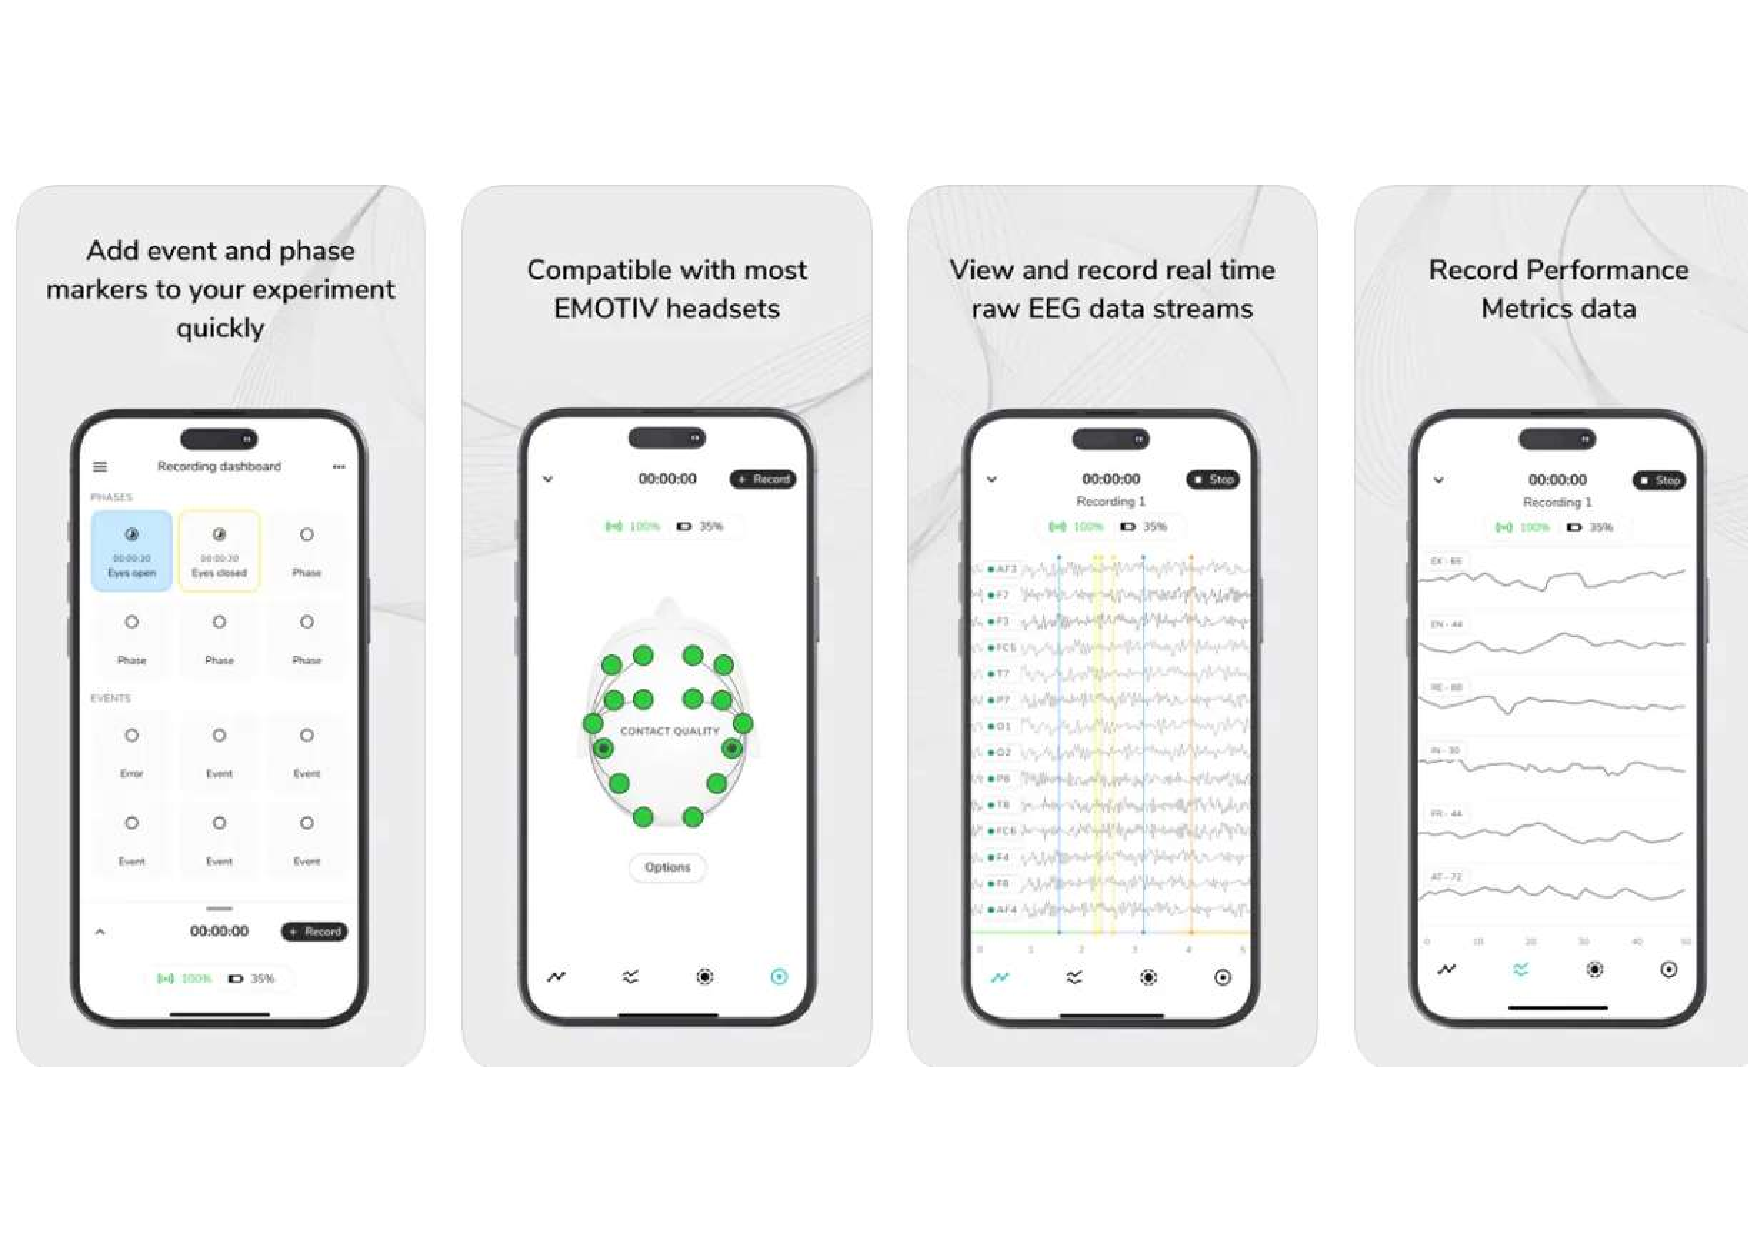
\includegraphics[width=0.8\textwidth]{img/CapturasEmotivPROMobile.pdf}
    \caption{Capturas de pantalla con el contenido de EmotivPRO Mobile.}
    \label{fig: CapturasEmotivPROMobile}
    \end{figure}
    \item PRO Tablet: Adquiere datos cerebrales contextuales con la aplicación de EEG PRO para tablets. Permite:
    \begin{itemize}
        \item Visualiza y graba datos EEG en bruto, métricas de rendimiento, datos de movimiento y más.
        \item Guardar tus datos en Emotiv Cloud para análisis posterior.
        \item Añade marcadores de eventos.
        \item Requiere Android 7.0 y superior o iOS 14.0 y superior. Para descargarlo en android se puede hacer a través de Play Store \cite{EmotivPROTabletAndroid}\footnote{Enlace de Play Store para descargar la aplicación de EmotivPRO para tablets \cite{EmotivPROTabletAndroid}.} y en la App Store en iOS \cite{EmotivPROTabletIOS}\footnote{Enlace de App Store para descargar la aplicación de EmotivPRO para tablets \cite{EmotivPROTabletIOS}.}.
    \end{itemize}
    \item PRO Desktop: Realiza investigaciones cerebrales exhaustivas con el \textit{software} de EEG PRO. Esta aplicación es más completa que las anteriores y permite:
    \begin{itemize}
        \item Diseñar experimentos de investigación.
        \item Obtener y grabar datos EEG en bruto, métricas de rendimiento, datos de movimiento y más.
        \item Guardar los datos localmente o en Emotiv Cloud para el análisis posterior.
        \item Analizar tus datos y mucho más
    \end{itemize}
\end{itemize}

\begin{table}[H]
\centering
\begin{tabular}{lcccc}
\rowcolor[HTML]{FFFFFF} 
Características & \multicolumn{4}{c}{\cellcolor[HTML]{FFFFFF}Versiones} \\
\rowcolor[HTML]{FFFFFF} 
 & \multicolumn{1}{l}{\cellcolor[HTML]{FFFFFF}Lite} & \multicolumn{1}{l}{\cellcolor[HTML]{FFFFFF}Standard} & \multicolumn{1}{l}{\cellcolor[HTML]{FFFFFF}Standard Team} & \multicolumn{1}{l}{\cellcolor[HTML]{FFFFFF}Performance} \\
\rowcolor[HTML]{FFFFFF} 
Datos EEG & \cellcolor[HTML]{FFFFFF}X & X & X & X \\
\rowcolor[HTML]{FFFFFF} 
Comandos mentales & X & X & X & X \\
\rowcolor[HTML]{FFFFFF} 
Grabaciones ilimitadas & \cellcolor[HTML]{FFFFFF}- & X & X & X \\
\rowcolor[HTML]{FFFFFF} 
Construir experimentos & \cellcolor[HTML]{FFFFFF}- & X & X & X \\
\rowcolor[HTML]{FFFFFF} 
Grabar, almacenar y exportar datos & \cellcolor[HTML]{FFFFFF}- & X & X & X \\
\rowcolor[HTML]{FFFFFF} 
Analizar datos post-procesados & \cellcolor[HTML]{FFFFFF}- & X & X & X \\
\rowcolor[HTML]{FFFFFF} 
\cellcolor[HTML]{FFFFFF}High Res Performance Metrics (2 Hz) & - & - & - & \cellcolor[HTML]{FFFFFF}X \\
\rowcolor[HTML]{FFFFFF} 
\cellcolor[HTML]{FFFFFF}Integración con D-LABS & - & - & - & \cellcolor[HTML]{FFFFFF}X \\
\rowcolor[HTML]{FFFFFF} 
\cellcolor[HTML]{FFFFFF}Lab Streaming Layer (LSL) & - & - & - & \cellcolor[HTML]{FFFFFF}X \\
\rowcolor[HTML]{FFFFFF} 
Límite de PC o MAC & 1 & 1 & 5 & 5
\end{tabular}
\caption{Tabla con la comparación de las distintas licencias de EmotivPRO.}
\label{tab:comparacionLicencias}
\end{table}

\subsubsection{Contour}
Es un \textit{software} integrado de Emotiv para la optimización del rendimiento cognitivo diario. Permite a los usuarios recopilar datos de EEG desde cualquier lugar y en cualquier momento, proporcionando análisis del estado cerebral en tiempo real \cite{Contour}\footnote{Página web oficial de Emotiv con la información correspondiente a Contour\cite{Contour}.}. Algunas características destacables que presenta son:
\begin{itemize}
    \item Información personalizada de la actividad cerebral: Aprovecha los algoritmos de aprendizaje automático y la inteligencia artificial de EMOTIV para proporcionar información personalizada sobre la actividad cerebral a lo largo del día.
    \item Optimización diaria: Cuando el usuario está estresado o pierde la concentración, Contour emite alertas y sugiere actividades que puedan ayudar al usuario.
    \item Compatibilidad: Está disponible en macOS (10.13) High Sierra o superior, Windows 10 (64 bits) v1809 o superior, Android 7.0 o superior e iOS 13 o superior.
\end{itemize}

Por lo tanto, Contour es una solución de \textit{software} de Emotiv que permite a los usuarios recopilar datos de EEG que permiten optimizar el rendimiento diario. Además, a medida que el usuario lo utiliza, se va adaptando a su actividad cerebral óptima. Si se tiene algún tipo de problema con esta aplicación, se puede consultar la página de Emotiv con ayuda sobre Contour \cite{ContourHelp}\footnote{Página web oficial de Emotiv con ayuda para la aplicación Contour\cite{ContourHelp}.}.

\subsection{Herramientas.}

En este apartado se presenta un resumen de las herramientas empleadas en el proyecto. Se han considerado diversas alternativas, destacando los aspectos más relevantes de cada una.

\subsubsection{Dispositivo Emotiv MN8.}
\textbf{Descripción.}
El MN8 es un dispositivo revolucionario que combina la comodidad de los auriculares con la potencia de la tecnología EEG de Emotiv \cite{EmotivMN8}\footnote{Sección de la página web oficial de Emotiv con toda la información correspondiente al dispositivo MN8 \cite{EmotivMN8}.}, presentando los siguientes aspectos clave:
\begin{enumerate}
    \item Diseño Innovador: Los auriculares EEG de 2 canales permiten escuchar música y monitorear las ondas cerebrales en cualquier momento y lugar. Su diseño discreto y cómodo se adapta al estilo de vida diario, pudiendo observarlo en la imagen \ref{fig: MN8}.
    \item Calidad de Datos: Los sensores EEG integrados capturan datos cerebrales de alta calidad de investigación mientras se realizan las actividades diarias, lo que brinda información valiosa sobre el cerebro y su funcionamiento.
    \item Funcionalidad Inteligente.
    \begin{itemize}
        \item Recargable. La batería tiene una duración de hasta 6 horas, lo que garantiza un uso prolongado sin preocupaciones.
        \item Configuración Rápida. Comienza a usarlo en menos de 1 minuto, sin complicaciones.
        \item Micrófono Integrado. Nunca pierdas una llamada mientras sigues monitoreando tu actividad cerebral.
    \end{itemize}
    \item Optimización Cognitiva con Contour:
    \begin{itemize}
        \item Carga Cognitiva. Mide el esfuerzo mental requerido para completar una tarea.
        \item Atención. Evalúa el enfoque vigilante durante las actividades.
        \item Estrés Cognitivo. Analiza el esfuerzo mental mientras se realizan tareas.
    \end{itemize}
\end{enumerate}

En resumen, el MN8 es mucho más que unos simples auriculares. Es una herramienta que permite comprender y mejorar la actividad cerebral.

\begin{figure}[H]
    \centering
    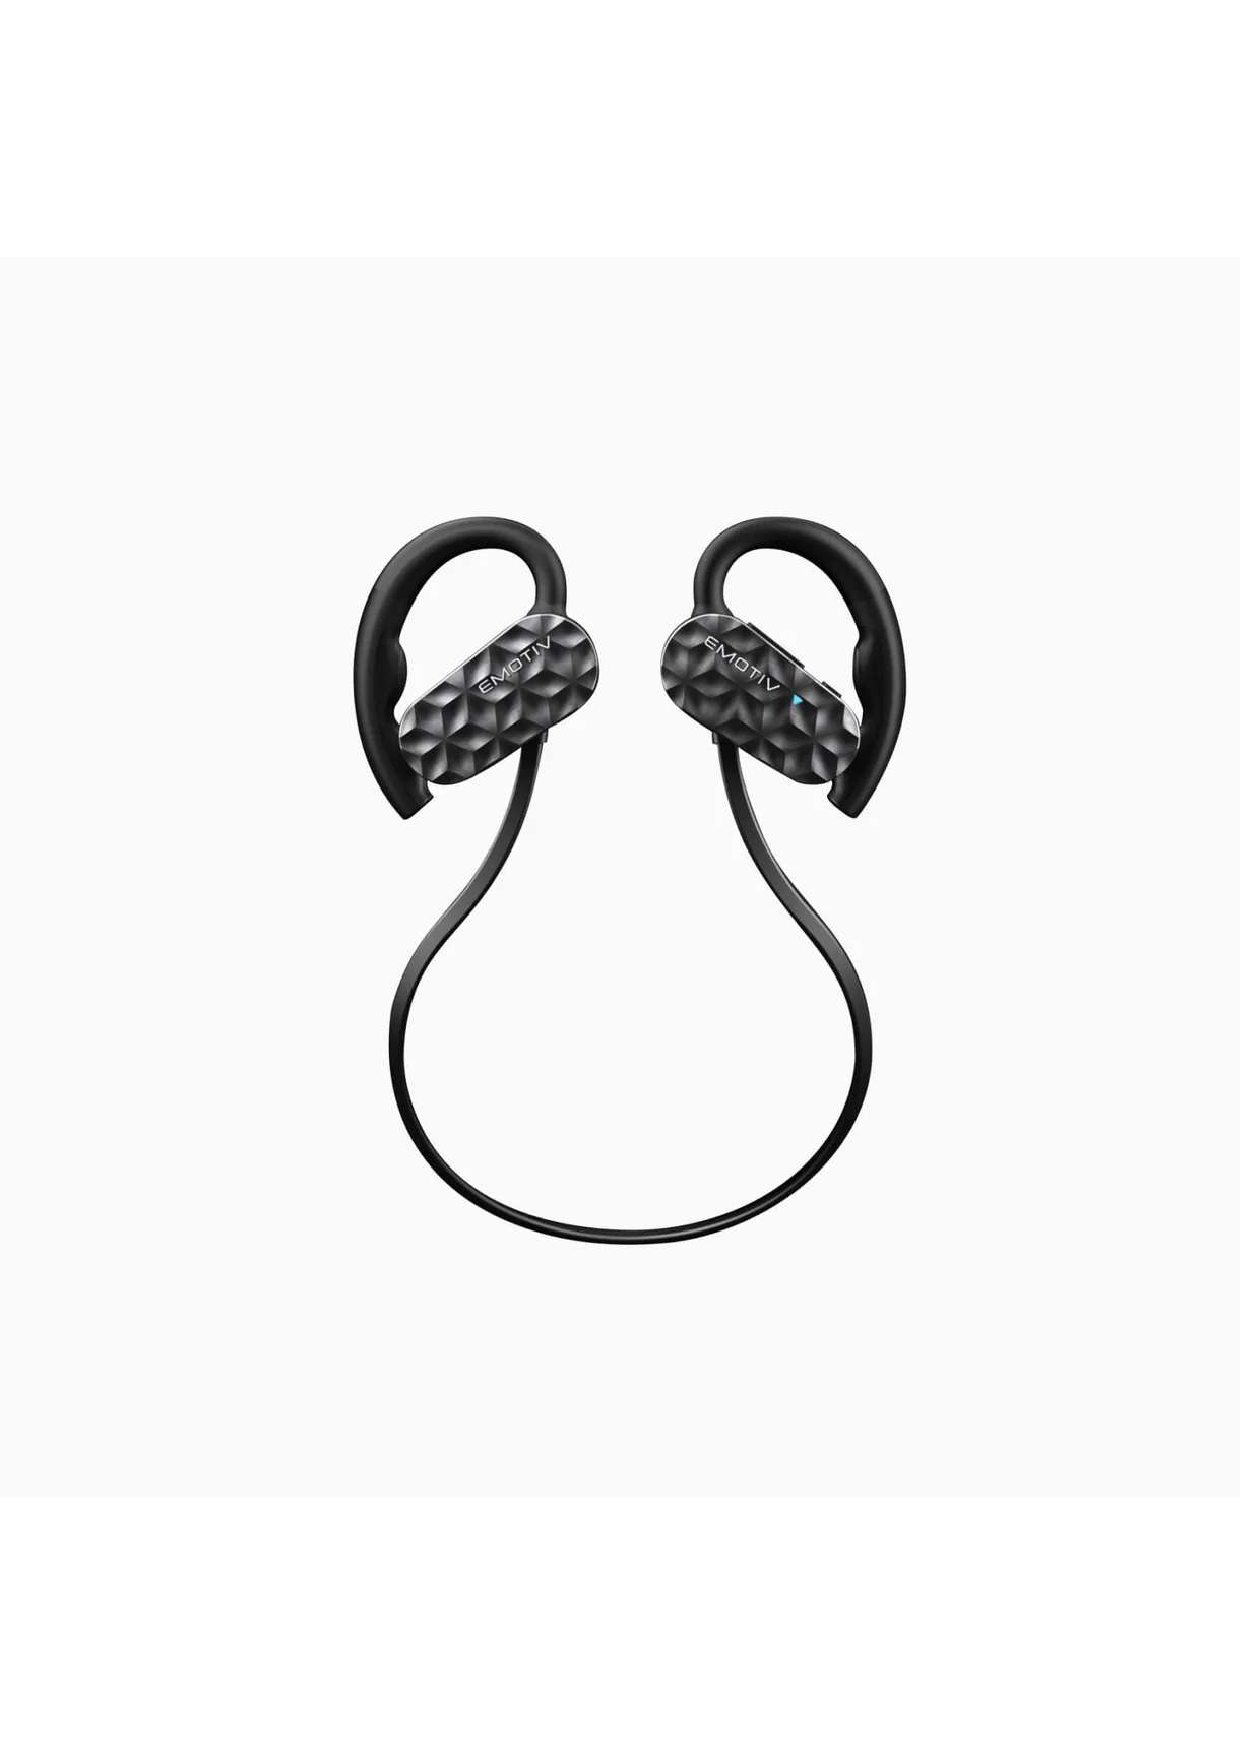
\includegraphics[width=0.4\textwidth]{img/MN8.pdf}
    \caption{Dispositivo MN8.}
    \label{fig: MN8}
\end{figure}

\textbf{Funcionamiento}
\begin{enumerate}
    \item Emparejar MN8 con Contour permite usar el MN8 y emparejarlo con Contour. Los sensores EEG integrados de MN8 miden sin problemas la actividad cerebral mientras se realizan actividades diarias.
    \item Mediciones inteligentes de la actividad cerebral. Para ello, Contour traduce los datos EEG de MN8 y utiliza IA y aprendizaje automático para proporcionar información personalizada sobre el cerebro y recomendaciones de actividad adaptadas al usuario.
    \item Su uso a diario permite que Contour se vuelva más inteligente cuanto más se usas, llegando a conocer la actividad cerebral óptima de cada usuario.
    \item Si el usuario está estresado o distraído, Contour alertará sobre los cambios en la actividad cerebral que están afectando a la eficiencia cognitiva. Sugerirá actividades para ayudar a desestresar o encontrar el flujo del usuario.
\end{enumerate}

\textbf{Especificaciones}
\begin{itemize}
    \item Cantidad de sensores. 2 (+4 referencias)
    \item Tecnología del sensor. Auriculares de elastómero conductor no tóxico, no alergénico y seco.
    \item Conectividad. Bluetooth 5.0 de baja energía.
    \item Ubicaciones del sensor. Canal auditivo izquierdo y derecho.
    \item Rango dinámico. ±4.17 mV.
    \item Resolución. 14 bits por canal.
    \item Resolución LSB. 0.51 µV.
    \item Aviso. No es compatible con Ubuntu y Raspberry Pi.
\end{itemize}

\textbf{Actividades}

Uno de los objetivos es replicar algunas de las cosas que hacen en Emotiv en el software de MN8. Para ello, se realizaron unas actividades durante 10 días para tratar de entender el cerebro y trabajar de manera más productiva. Tras completar este entrenamiento, los expertos analizan los datos y entregan informes personalizados, que muestran cómo el cerebro se ve afectado por técnicas de bienestar y permite la comparación con otros participantes del proyecto.

Para este procedimiento, cada día se comienza con un ejercicio de cerebro en reposo, seguido de un ejercicio de respiración o de meditación consciente en función del día. Inmediatamente después de eso, se realizará una sesión de concentración en la aplicación Contour. Después de cada día se recibirá un email de Emotiv que contiene un link con algunas preguntas sobre la satisfacción de la experiencia.

Tras completar todo el ciclo de actividades (10 días), se analizarán los datos y se generará un informe individual. Los datos permanecerán anónimos y cada persona únicamente verá sus propios resultados individuales y además, datos de otros miembros de la comunidad de manera anónima. Por lo tanto, las actividades que se realizarán son \cite{actividades}\footnote{Página web de Emotiv en la que se detallan las distintas actividades indicadas\cite{actividades}.}:
\begin{itemize}
    \item Ejercicios en reposo.
    \begin{itemize}
        \item Este tipo de ejercicios proporciona una idea de cómo se ve el cerebro cuando la persona no hace nada, lo que permite comparar la actividad cerebral durante otras tareas (como sesiones de concentración). De esta manera, se puede decir si al realizar una actividad, el estado cerebral ha cambiado significativamente. Las grabaciones de EEG en estado de reposo se utilizan comúnmente en la investigación de neurociencia.
        \item Dentro de estos ejercicios, se realizarán 2 tipos distintos:
        \begin{itemize}
            \item 15 segundos con ojos abiertos, indicando las zonas de concentración.
            \item 15 segundos con ojos cerrados, indicando las zonas de concentración junto con el aviso de inicio y final.
        \end{itemize}
    \end{itemize}
    \item Ejercicios de respiración o meditación.
    \begin{itemize}
        \item Dependiendo del día u objetivo, se pueden realizar ejercicios de respiración o de meditación. Dentro de la aplicación, se puede seleccionar cuál de ellos se desea realizar.
    \end{itemize}
    \item Ejercicios de concentración y mindfulness
        \begin{itemize}
            \item Se realizan sesiones de concentración, cuya duración puede ser cambiada en función de las necesidades y además permite detener manualmente la sesión.
        \end{itemize}
    \item Ejercicios de concentración, círculos y similares.
        \begin{itemize}
            \item Se pueden realizar tantas sesiones de concentración como el usuario desee, lo que permite que, a mayor número de sesiones, mayor información proporcionarán los datos.
        \end{itemize}
\end{itemize}

\subsection{Comparación de entornos y herramientas.}

\subsubsection{Ventajas del uso de PsychoPy con Emotiv}
PsychoPy es una plataforma de código abierto que permite la creación de experimentos en neurociencia cognitiva. Cuando se utiliza en combinación con dispositivos de Emotiv, ofrece varias ventajas\cite{EMOTIVDevelopers}\footnote{Página web de Emotiv en la que se detalla información para el desarrollo de aplicaciones con Emotiv \cite{EMOTIVDevelopers}.}:

\begin{itemize}
    \item Interfaz gráfica intuitiva. Ofrece una interfaz gráfica de usuario (GUI) en su vista de Builder que facilita la creación de experimentos sin necesidad de programar. Gracias a ello, los investigadores pueden diseñar su experimento arrastrando y soltando componentes visuales y temporales en una cuadrícula visual. Esto es útil para aquellos que no tienen experiencia en programación.
    \item Facilidad de uso. Simplifica la creación de paradigmas experimentales al proporcionar una interfaz intuitiva. Los investigadores pueden centrarse en el diseño y la lógica del experimento sin preocuparse por la implementación técnica. Además, no se requieren conocimientos avanzados de programación para utilizar PsychoPy.
    \item Compatibilidad con dispositivos EEG. Admite la integración con dispositivos EEG, incluyendo entre ellos el EMOTIV MN8. El componente ‘Emotiv Marking’ permite enviar marcadores al flujo de datos EEG en el momento en que se presentan los estímulos \cite{psychopyEmotivMarking}\footnote{Página web oficial de PsychoPy que contiene explicaciones de marcadores \cite{psychopyEmotivMarking}.}. Estos marcadores son cruciales para identificar eventos específicos en los datos EEG. El ‘Emotiv Marking’ se conecta al auricular Emotiv para enviar marcadores al flujo de datos, lo que garantiza una sincronización precisa.
    \item Marcadores precisos y sincronización temporal. Asegura que los marcadores se envíen con precisión al auricular Emotiv MN8 en el momento adecuado durante la presentación de estímulos. Los marcadores pueden etiquetarse y contener valores específicos, lo que facilita la identificación de eventos en los datos EEG recopilados. La sincronización temporal es crucial en experimentos neurocientíficos, y PsychoPy se encarga de esta tarea de manera fiable.
    \item Exportación a otros formatos y plataformas. Aunque los componentes emotiv no funcionan en Pavlovia (la plataforma de PsychoPy para experimentos en línea), es posible exportar el experimento a HTML y luego importarlo en Emotiv OMNI para su análisis posterior. Esto permite a los investigadores trabajar con los datos recopilados utilizando las herramientas específicas de EMOTIV.
    \item Flexibilidad en la programación. Permite a los investigadores escribir código personalizado en Python dentro de sus experimentos. Resulta útil cuando se requiere una lógica más compleja o cuando se necesita personalizar el flujo del experimento. Los usuarios pueden combinar componentes visuales y temporales con código Python, lo que brinda una mayor flexibilidad en la programación.
\end{itemize}
    
Por lo tanto, trabajar con PsychoPy ofrece una solución completa y amigable para diseñar y ejecutar experimentos que involucren el dispositivo EMOTIV MN8, garantizando una integración precisa y una experiencia de desarrollo eficiente.

Por otro lado, trabajar con PsychoPy también presenta algunas limitaciones a tener en cuenta:
\begin{itemize}
    \item Velocidad de marcadores. El componente Emotiv Marking en PsychoPy envía marcadores al flujo de datos EEG en el momento en que se presentan los estímulos. Sin embargo, si se necesitan velocidades de marcadores más altas que las proporcionadas por defecto (aproximadamente 0.2 segundos), es mejor registrar manualmente los tiempos de los marcadores y compararlos con los tiempos en los datos EEG crudos \cite{psychopyEmotivMarking}\footnote{Sección de la página web oficial de PsychoPy con información sobre el 'Emotiv Marking Component' \cite{psychopyEmotivMarking}.}.
    \item Exportación a Pavlovia. Si se exporta el experimento a HTML para ejecutarlo en la plataforma en línea Pavlovia, los componentes emotiv no tendrán efecto. Para analizar los datos recopilados en Emotiv OMNI, debes seguir las instrucciones para importar el experimento desde HTML en la plataforma OMNI \cite{pavlovia}\footnote{Página web oficial de Pavlovia que con toda la información referida a ella \cite{pavlovia}.}.
\end{itemize}

\subsubsection{Compatibilidad entre \textit{Eye tracking} y PsychoPy.}
Una gran diferencia entre la API de Emotiv y PsychoPy  es que este último permite la inclusión de otros dispositivos para la realización de distintos experimentos. Para este proyecto, puede ser interesante la inclusión de un dispositivo \textit{eye tracking}, cuya implementación y características se encuentran descritas en un artículo titulado 'Communicating with an Eyetracker — PsychoPy v2024.1.4' \cite{PsychoPyEyeTracking}\footnote{Sección de la página oficial de PsychoPy con la descripción de los pasos para comunicar el \textit{eye tracking} con PsychoPy \cite{PsychoPyEyeTracking}.}.

Este artículo proporciona una guía detallada sobre cómo utilizar la aplicación PsychoPy para interactuar con los \textit{eye trackers}. Como ya se ha explicado anteriormente, PsychoPy es una plataforma de código abierto para la neurociencia cognitiva que tiene componentes incorporados que permiten la comunicación directa con los \textit{eye trackers}.

Estos componentes permiten a los usuarios configurar, calibrar y grabar datos de \textit{eye tracking} directamente desde el Builder de PsychoPy, sin necesidad de escribir código. PsychoPy es compatible con una variedad de eyetrackers comúnmente utilizados, y los usuarios pueden verificar la compatibilidad de su dispositivo a través de la interfaz de la aplicación.

Además, para los usuarios que deseen probar experimentos de \textit{eye tracking} pero no tengan un \textit{eye tracker}, PsychoPy ofrece la opción MouseGaze. Esta opción permite que el cursor del ratón actúe como un punto de mirada, simulando movimientos oculares sin la necesidad de un \textit{eye tracker}.

Por lo tanto, este artículo proporciona una visión valiosa para cualquier proyecto que busque incorporar \textit{eye tracking} en sus experimentos utilizando PsychoPy. Su enfoque en la facilidad de uso y la compatibilidad con una variedad de dispositivos hace de PsychoPy una opción atractiva para los investigadores en este campo.

\subsubsection{Compatibilidad entre Tobii y PsychoPy.}
PsychoPy es compatible con varios dispositivos de \textit{eye tracking} de Tobii. Aunque la documentación específica no menciona las versiones exactas de los dispositivos de Tobii que son compatibles, hay evidencias de la compatibilidad con varios modelos \cite{TobiiPsychoPy}\footnote{Página web oficial de PsychoPy que contiene información de cómo realizar la conexión con el \textit{eye tracking} Tobii y los elementos utilizables dentro del entorno \cite{TobiiPsychoPy}.}. 

Uno de los modelos mencionados en la comunidad de usuarios de PsychoPy es el Tobii Pro X3-120 \cite{ForoTobiiPsychoPy}\footnote{Foro de PsychoPy en el que los usuarios comparten información, problemas y soluciones \cite{ForoTobiiPsychoPy}.}. Este dispositivo de \textit{eye tracking} es conocido por su alta frecuencia de muestreo y precisión, lo que lo hace adecuado para una variedad de investigaciones en el campo de la psicología y la neurociencia.

Además, en la página oficial de PsychoPy se menciona el uso de otros dispositivos de Tobii como el Tobii Pro Nano, Tobii Pro Fusion, Tobii Pro Spectrum, y Tobii TX300 \cite{SupportTobii}\footnote{Página oficial de Tobii que contiene los \textit{eye trackings} compatibles \cite{SupportTobii}.}. Estos dispositivos también podrían ser empleados con PsychoPy, ampliando así las opciones disponibles para los investigadores.

Se recomienda el uso del \textit{software} gratuito Eyetracker Manager de Tobii para asegurarse de que el dispositivo Tobii está conectado y funcionando correctamente antes de iniciar cualquier experimento con PsychoPy.

Para utilizar dispositivos Tobii con PsychoPy, se describe una caja de herramientas llamada Titta. Titta es una caja de herramientas de Python (PsychoPy) y Matlab (PTB) que permite comunicarse con los \textit{eye trackers} de Tobii.

Es importante tener en cuenta que la compatibilidad puede variar dependiendo de la versión de PsychoPy que se esté utilizando. Por lo tanto, se recomienda consultar la documentación oficial de PsychoPy para obtener la información más actualizada.

\subsection{Comparación de Emotiv con Métodos Anteriores.}

Antes de la existencia de dispositivos como el MN8, la medición de la concentración, el estrés y la carga cognitiva solía ser subjetiva \cite{ArticuloMedicionCG}\footnote{Artículo que trata la carga mental y cómo se mide \cite{ArticuloMedicionCG}.}. Se utilizaban encuestas, cuestionarios o entrevistas para obtener información de las personas, pero esto tenía limitaciones:
\begin{itemize}
    \item Subjetividad: Las respuestas podían estar influenciadas por la percepción individual y no siempre eran precisas.
    \item Limitaciones de la comunicación verbal: No siempre se podía expresar completamente el estado mental.
    \item Falta de objetividad: No se basaba en mediciones directas del cerebro.
\end{itemize}

En resumen, el MN8 utiliza sensores EEG y métricas de rendimiento para evaluar la concentración, el estrés y la carga cognitiva de manera más objetiva y precisa que los métodos anteriores basados en encuestas y subjetividad \cite{EncuestaNivelEstres}\footnote{Página de la OCU con una encuesta para saber los niveles de estrés del participante \cite{EncuestaNivelEstres}.}.

\subsection{Comparación de MN8 con otros dispositivos.}
En este apartado, se realizará un análisis de tres productos de neurotecnología de Emotiv: el MN8, el Insight y el EPOC X. Aunque todos estos dispositivos tienen el objetivo común de capturar y analizar datos de EEG, presentan diferencias significativas en términos de diseño, funcionalidad y aplicaciones.

El MN8 está diseñado para mejorar la productividad y el bienestar, el Insight proporciona información sobre el estado mental del usuario y el EPOC X se utiliza en la investigación y las aplicaciones de BCI \cite{comparacionHeadsets}\footnote{En la página web de Emotiv se describen detalladamente las características de cada dispositivo \cite{comparacionHeadsets}.}.

\subsubsection{Emotiv Insight}
Es un auricular EEG inalámbrico de 5 canales creado por Emotiv que se puede ver en la imagen \ref{fig: Insight}. Se trata de una herramienta que permite capturar datos de las ondas cerebrales sin necesidad de gel o solución salina, posibilitando la observación del estado mental en tiempo real. Además, es ideal para explorar aplicaciones de control mental y tecnología asistida \cite{EmotivInsight}\footnote{Sección de la página web oficial de Emotiv con toda la información correspondiente al dispositivo Insight \cite{EmotivInsight}.}.

En comparación con el MN8, ambos son dispositivos EEG de alta calidad, pero tienen algunas diferencias clave que pueden hacer que uno sea más ventajoso que el otro dependiendo de tus necesidades. Las principales ventajas del MN8 sobre el Insight son:

\begin{enumerate}
    \item Diseño de auriculares. A diferencia del Insight, el MN8 es más compacto y discreto, lo que lo hace ideal para mediciones prolongadas e inadvertidas. Su diseño permite que se ubique directamente en la oreja, lo que lo hace menos visible y más cómodo para el uso a largo plazo de los usuarios.
    \item Audio de alta calidad. A diferencia del Insight, el MN8 permite escuchar música, podcasts, audiolibros y más mientras monitoreas la actividad cerebral.
    \item Micrófono integrado. El MN8 tiene un micrófono integrado, lo que permite continuar monitoreando la actividad cerebral durante las llamadas telefónicas y las reuniones.
    \item Compatibilidad con Contour. Los MN8 se pueden emparejar con Contour, una aplicación que proporciona retroalimentación en tiempo real sobre la actividad cerebral mientras se trabaja, escucha música, medita y más. Contour utiliza algoritmos de aprendizaje automático y IA de Emotiv para proporcionar información personalizada sobre la actividad cerebral a lo largo del día.
\end{enumerate}

Es importante tener en cuenta que la elección entre el MN8 y el Insight depende de las necesidades y preferencias individuales.

\begin{figure}[H]
    \centering
    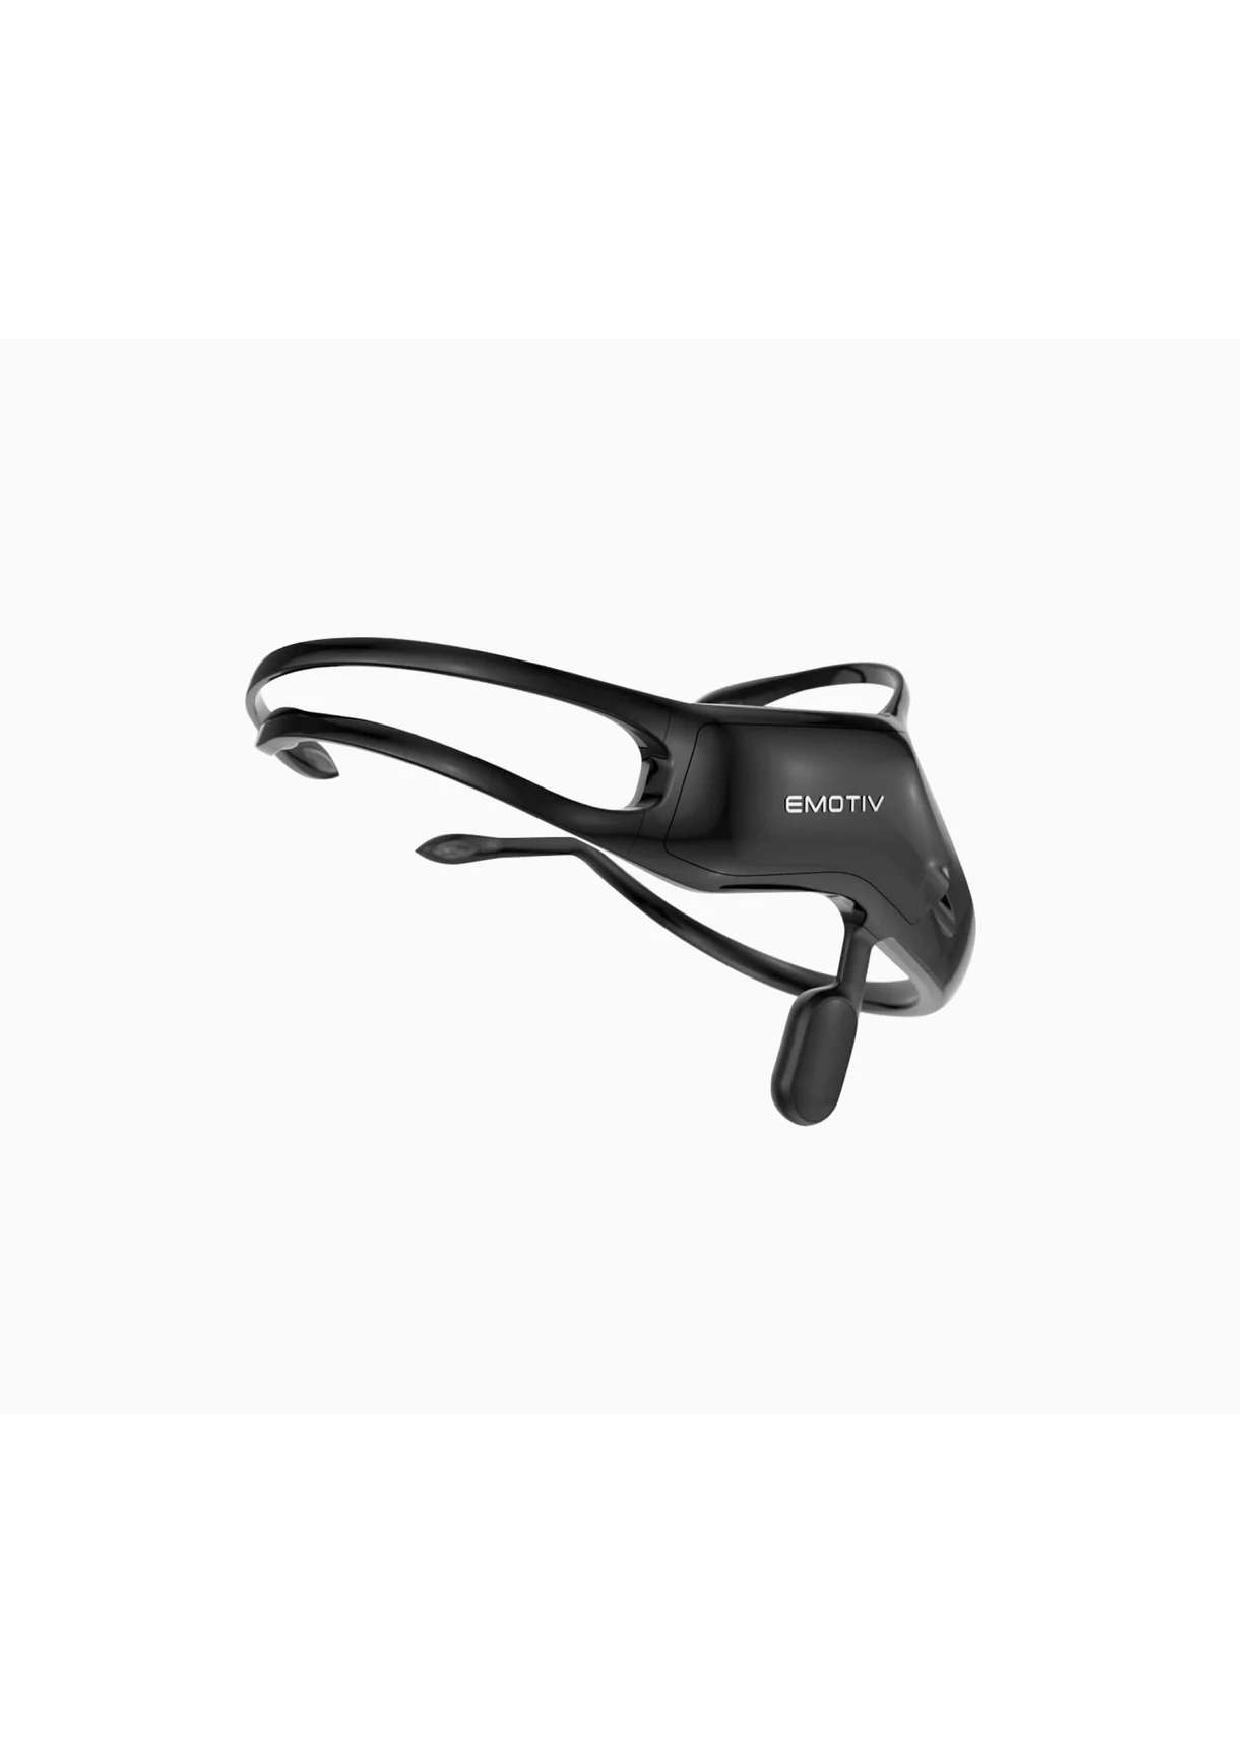
\includegraphics[width=0.4\textwidth]{img/Insight.pdf}
    \caption{Dispositivo Insight.}
    \label{fig: Insight}
\end{figure}

\subsubsection{Emotiv EPOCX}
Dispositivo diseñado por Emotiv para investigaciones cerebrales humanas escalables \cite{EmotivEPOCX}\footnote{Sección de la página web oficial de Emotiv con toda la información correspondiente al dispositivo Insight \cite{EmotivEPOCX}.}. Posee 14 canales de EEG y sensores basados en solución salina que proporcionan acceso a datos cerebrales de calidad profesional, puediendo observar su diseño en la imagen \ref{fig: EPOC X}. Su conectividad inalámbrica lo hace ideal para estudios científicos y aplicaciones de neurociencia, ya que ofrece una visión profunda del cerebro humano y su actividad.

El Emotiv MN8 y el Emotiv EPOCX son dispositivos EEG de alta calidad, pero tienen algunas diferencias clave que pueden hacer que uno sea más ventajoso que el otro dependiendo de tus necesidades. Las ventajas del MN8 sobre el EPOCX son:

\begin{enumerate}
    \item Diseño de auriculares. A diferencia del EPOCX, el MN8 es más compacto y discreto, lo que lo hace ideal para mediciones prolongadas e inadvertidas. Su diseño permite que se ubique directamente en la oreja, lo que lo hace menos visible y más cómodo para el uso a largo plazo de los usuarios.
    \item Audio de alta calidad y micrófono integrado. El MN8 permite escuchar música, podcasts, audiolibros y más mientras monitorea la actividad cerebral. Además, tiene un micrófono integrado, lo que te permite continuar monitoreando la actividad cerebral durante las llamadas telefónicas y las reuniones. Estas características no están disponibles en el EPOCX.
    \item Compatibilidad con Contour. Los MN8 se pueden emparejar con Contour \cite{Contour}\footnote{Página web oficial de Emotiv con la información correspondiente a Contour\cite{Contour}.}, una aplicación que proporciona retroalimentación en tiempo real sobre la actividad cerebral mientras el usuario trabaja, escucha música, medita o realiza otro tipo de actividades. Contour utiliza algoritmos de aprendizaje automático y AI de Emotiv para proporcionar información personalizada sobre la actividad cerebral a lo largo del día. Esta característica no está disponible en el EPOCX.
    \item Facilidad de uso. El MN8 es fácil de usar y configurar, lo que puede ser una ventaja sobre el EPOCX, que puede requerir una configuración más compleja. Además, aunque el MN8 tiene menos sensores que el Insight y el EPOCX, utiliza una tecnología de sensor seco no tóxico y no alergénico, lo que puede ser una ventaja para aquellos con sensibilidades de piel o alergias.
    \item Conectividad y Batería. El MN8 ofrece conectividad a través de \textit{Bluetooth Low Energy}, lo que puede ser más conveniente para algunos usuarios en comparación con el receptor USB propietario requerido por el Insight y el EPOCX. Además, aunque la vida útil de la batería del MN8 es menor que la del Insight y el EPOCX, sigue siendo suficiente para muchas aplicaciones con hasta 6 horas de duración.
\end{enumerate}

Al igual que con el Emotiv Insight, hay que tener en cuenta que la elección entre el MN8 y el EPOCX dependerá de las necesidades y preferencias de cada usuario, ya que ambos ofrecen una gama de características y ventajas únicas.

\begin{figure}[H]
    \centering
    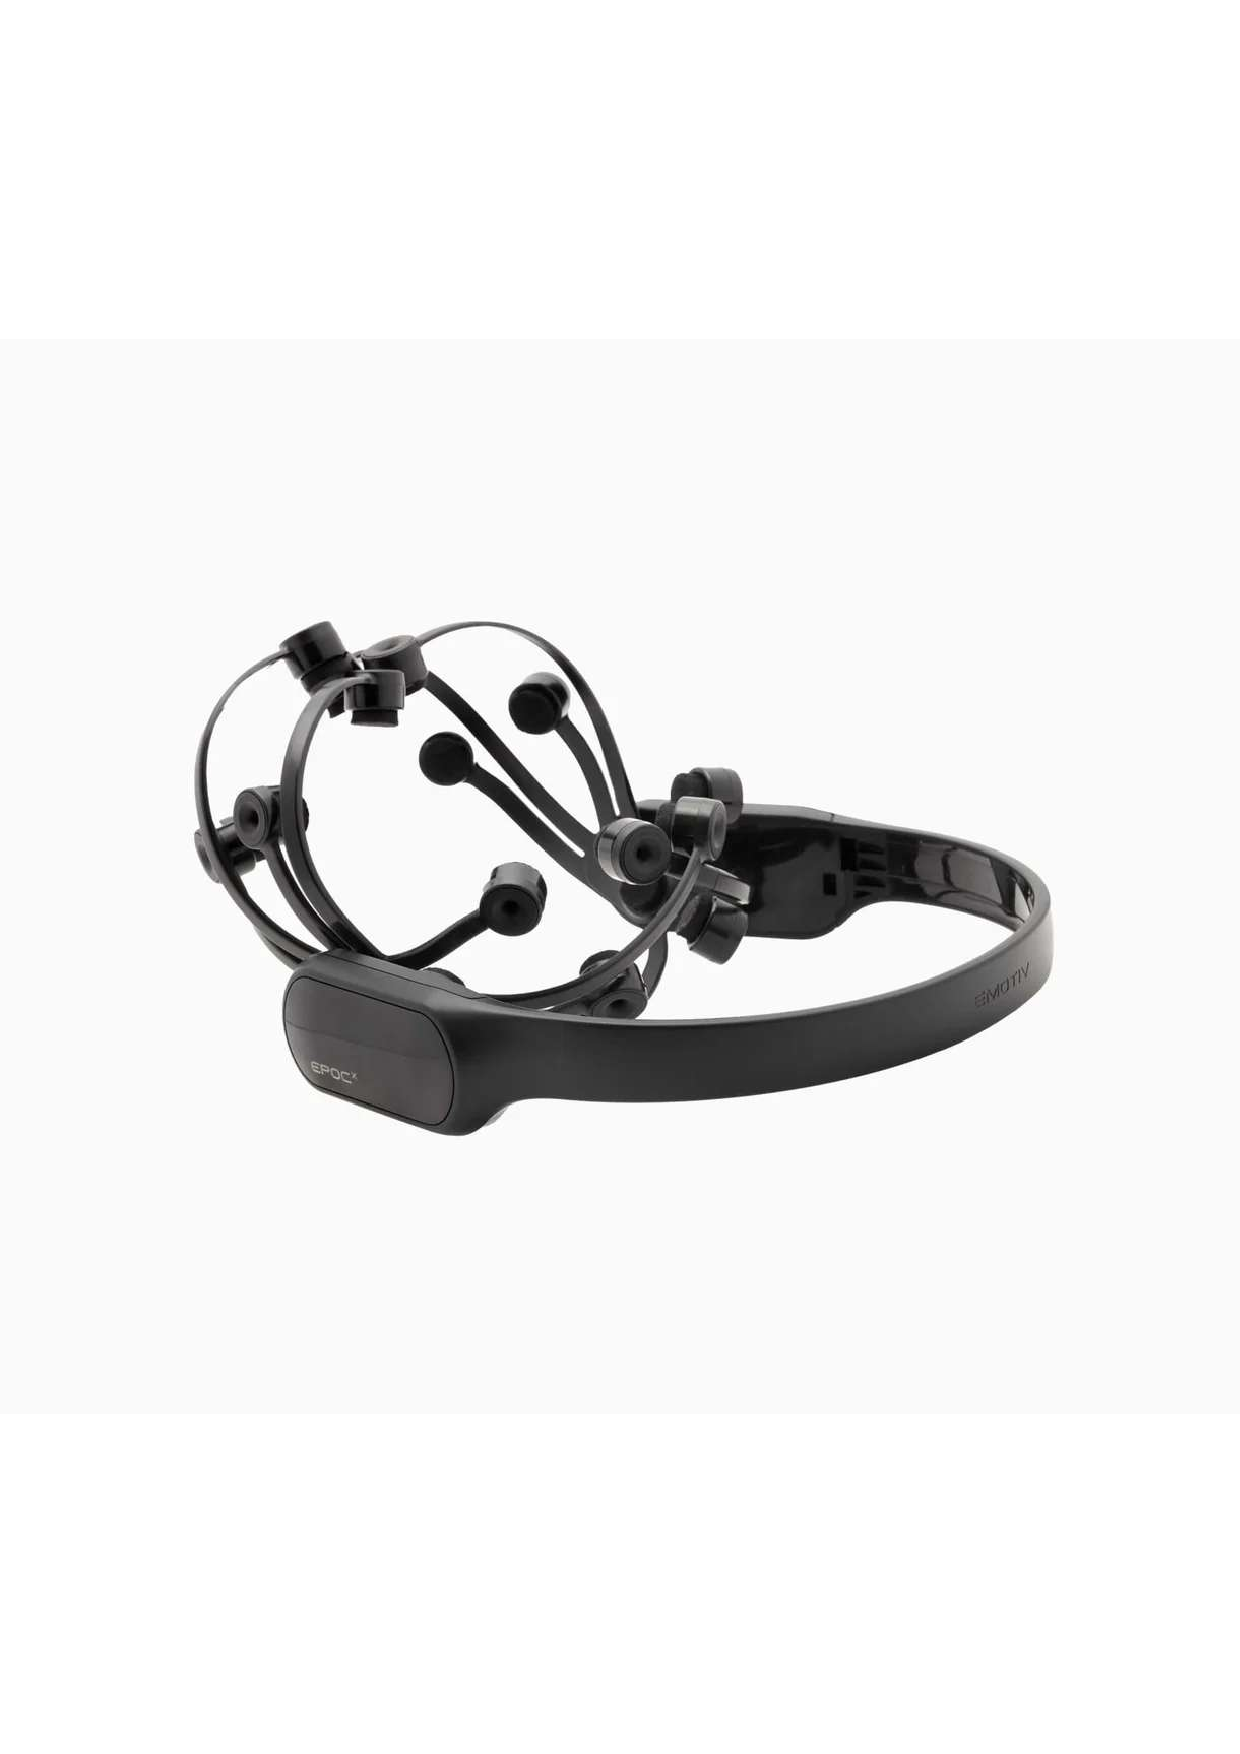
\includegraphics[width=0.4\textwidth]{img/EPOCX.pdf}
    \caption{Dispositivo EPOC X.}
    \label{fig: EPOC X}
\end{figure}

\subsubsection{Conclusiones de la comparación entre los dispositivos de Emotiv.}
El Emotiv MN8 destaca por su diseño compacto y discreto, lo que lo hace ideal para mediciones prolongadas sin causar molestias. Aunque tiene menos sensores que el Insight y el EPOCX, su tecnología de sensor seco no tóxico y su conectividad Bluetooth Low Energy lo hacen atractivo. Además, se espera que el MN8 mida el estrés cognitivo y la concentración, lo que amplía sus posibilidades de uso.

Por otro lado, el Insight y el EPOCX ofrecen más sensores y opciones de medición, lo que los hace ideales para investigaciones más avanzadas o aplicaciones clínicas. La elección dependerá de las necesidades de cada usuario y el objetivo de su uso. Por lo tanto, el MN8 es una opción discreta y tecnológicamente avanzada, mientras que el Insight y el EPOCX son más versátiles en términos de medición cerebral. Estas comparaciones se pueden ver de manera más clara en la tabla \ref{tab:comparacionHeadsetsEmotiv}, obtenida a partir de la página web de Emotiv en la sección de \textit{comparision} \cite{comparacionHeadsets}\footnote{Sección de comparación de los dispositivos de Emotiv dentro de su página oficial \cite{comparacionHeadsets}.}.

\begin{table}[]
\centering
\resizebox{15cm}{!}{
\begin{tabular}{|l|c|c|c|}
\hline
\rowcolor[HTML]{EFEFEF} 
\textbf{Características} & \textbf{Insight} & \textbf{EPOC X} & \textbf{MN8} \\ \hline
\rowcolor[HTML]{FFFFFF} 
{\color[HTML]{111111} \begin{tabular}[c]{@{}l@{}}Número\\ de sensores\end{tabular}} & {\color[HTML]{111111} 5 (+2 referencias)} & {\color[HTML]{111111} 14 (+2 referencias)} & {\color[HTML]{111111} 2 (+4 referencias)} \\ \hline
\rowcolor[HTML]{FFFFFF} 
{\color[HTML]{111111} \begin{tabular}[c]{@{}l@{}}Posición\\ de sensores\end{tabular}} & \cellcolor[HTML]{FFFFFF}{\color[HTML]{111111} \begin{tabular}[c]{@{}c@{}}AF3, AF4, \\ T7, T8, Pz\end{tabular}} & {\color[HTML]{111111} \begin{tabular}[c]{@{}c@{}}AF3, AF4, F3, \\ F4, FC5, FC6,\\ F7, F8, T7, \\ T8, P7, P8, O1, O2\\ (configurable en cualquier \\ ubicación 10-20)\end{tabular}} & {\color[HTML]{111111} \begin{tabular}[c]{@{}c@{}}Canal auditivo izquierdo\\ y derecho\end{tabular}} \\ \hline
\rowcolor[HTML]{FFFFFF} 
{\color[HTML]{111111} Resolución} & {\color[HTML]{111111} \begin{tabular}[c]{@{}c@{}}16 bits por \\ canal\end{tabular}} & {\color[HTML]{111111} \begin{tabular}[c]{@{}c@{}}14 bits o 16 bits \\ por canal (configurable por \\ el usuario)\end{tabular}} & {\color[HTML]{111111} 14 bits por canal} \\ \hline
\rowcolor[HTML]{FFFFFF} 
{\color[HTML]{111111} \begin{tabular}[c]{@{}l@{}}Tecnología\\ del sensor\end{tabular}} & \cellcolor[HTML]{FFFFFF}{\color[HTML]{111111} \begin{tabular}[c]{@{}c@{}}Polímero semiseco \\ de larga duración\end{tabular}} & {\color[HTML]{111111} \begin{tabular}[c]{@{}c@{}}Almohadillas empapadas \\ en solución salina o \\ Ag/AgCl + gel\end{tabular}} & {\color[HTML]{111111} \begin{tabular}[c]{@{}c@{}}Elastómero conductor no\\ tóxico y no alergénico\end{tabular}} \\ \hline
\rowcolor[HTML]{FFFFFF} 
{\color[HTML]{111111} Conectividad} & \cellcolor[HTML]{FFFFFF}{\color[HTML]{111111} \begin{tabular}[c]{@{}c@{}}Bluetooth® de \\ baja energía\end{tabular}} & {\color[HTML]{111111} \begin{tabular}[c]{@{}c@{}}Bluetooth® de \\ baja energía\end{tabular}} & {\color[HTML]{111111} \begin{tabular}[c]{@{}c@{}}Bluetooth® de\\ baja energía\end{tabular}} \\ \hline
\rowcolor[HTML]{FFFFFF} 
{\color[HTML]{111111} \begin{tabular}[c]{@{}l@{}}Duración de\\ la batería\end{tabular}} & \cellcolor[HTML]{FFFFFF}{\color[HTML]{111111} Hasta 20 horas} & {\color[HTML]{111111} Hasta 9 horas} & {\color[HTML]{111111} Hasta 6 horas} \\ \hline
\rowcolor[HTML]{FFFFFF} 
{\color[HTML]{111111} \begin{tabular}[c]{@{}l@{}}Frecuencia\\ de muestreo\end{tabular}} & \cellcolor[HTML]{FFFFFF}{\color[HTML]{111111} \begin{tabular}[c]{@{}c@{}}2048 (reducido \\ a 128 SPS)\end{tabular}} & {\color[HTML]{111111} \begin{tabular}[c]{@{}c@{}}2048 (reducido a 128 \\ SPS o 256 SPS,\\ configurable por el usuario)\end{tabular}} & {\color[HTML]{111111} \begin{tabular}[c]{@{}c@{}}2048\\ (reducido a 256 SPS)\end{tabular}} \\ \hline
\rowcolor[HTML]{FFFFFF} 
\cellcolor[HTML]{FFFFFF}{\color[HTML]{111111} Detecciones} & {\color[HTML]{111111} \begin{tabular}[c]{@{}c@{}}Parpadeo, guiño, \\ ceño fruncido,\\ sonrisa, apretar los dientes\end{tabular}} & {\color[HTML]{111111} \begin{tabular}[c]{@{}c@{}}Parpadeo, guiño,\\ mirar a izquierda/derecha,\\ ceño fruncido, sonrisa,\\ apretar los dientes, reír, mueca\end{tabular}} & {\color[HTML]{111111} \begin{tabular}[c]{@{}c@{}}Parpadeo, guiño,\\ mirar a izquierda/derecha,\\ ceño fruncido, sonrisa,\\ apretar los dientes, reír, mueca\end{tabular}} \\ \hline
\end{tabular}
}
\caption{Tabla con la comparación de los distintos 'Headsets' de Emotiv.}
\label{tab:comparacionHeadsetsEmotiv}
\end{table}

\capitulo{5}{Resultados}

\section{Resumen de resultados.}

Breve resumen de los resultados. En caso de ser un trabajo muy experimental, los resultados completos pueden aparecer en su anexo correspondiente.

Debería haber una correspondencia entre los objetivos y los resultados explicados en esta sección

\section{Discusión.}

Discusión y análisis de los resultados obtenidos.

\capitulo{6}{Conclusiones}

En este proyecto, se han logrado alcanzar los objetivos planteados mediante un enfoque metódico y colaborativo. Los objetivos conseguidos son:
\begin{itemize}
    \item Comprender el funcionamiento del dispositivo Emotiv MN8 y para ello, se ha realizado una investigación profunda sobre el dispositivo y varias pruebas para entender completamente cómo funciona.
    \item Familiarizarse con los métodos de recopilación y análisis y para ello se han realizado varias pruebas con las aplicaciones de Contour y Emotiv, concretamente Emotiv Labs.
    \item Diseñar y realizar una serie de experimentos en el entorno de PsychoPy y para ello se ha tratado de emplear el PsychoPy Coder, pero se han experimentado muchos problemas y no se puede conseguir un resultado válido. Por lo tanto, se ha utilizado el PsychoPy Builder, permitiendo el diseño del experimento de una forma más sencilla.
    \item Evaluar la validez del dispositivo MN8 para su uso en el ámbito sanitario, el cual no se ha realizado específicamente pero hay estudios y artículos que indican la validez de los dispositivos Insight y EPOC X en este ámbito, lo que sugiere que los datos recopilados por el MN8 también son válidos.
    \item Contribuir a la comprensión de cómo se pueden utilizar los dispositivos EEG portables en la práctica sanitaria. Para ello, se ha realizado una investigación profunda sobre el dispositivo, aplicaciones y limitaciones entre otras cosas.
    \item Usar las herramientas de GitHub y Overleaf durante el desarrollo del proyecto, permitiendo un seguimiento y realización de toda la documentación del TFG.
    \item Analizar costes y viabilidad legal y para ello se ha realizado una investigación de todos los componentes necesarios así como las leyes que pueden afectar al proyecto.
    \item Realizar un trabajo reproducible en el futuro. Para hacer esto posible, se ha realizado la documentación de la forma más clara y explicativa posible, tanto de Emotiv como de PsychoPy.
\end{itemize}

\section{Aspectos relevantes.}

Este apartado pretende recoger los aspectos más interesantes del desarrollo del proyecto, incluyendo los detalles más relevantes en cada fase del desarrollo, justificando los caminos tomados, especialmente aquellos que no sean triviales. Hay que tener en cuenta que estos problemas o modificaciones producidas pueden haber sido causados por las características de los materiales antialérgenos o su tratamiento, ya que en otros dispositivos, como los del laboratorio, no ha sido necesario.

\subsection{Problemas de conexión intermitente con Emotiv Insight.}
\subsubsection{Descripción del problema.}
Durante la semana del Objetivo 5, mientras realizaba el proceso de conexión del Emotiv Insight con el ordenador, he experimentado un problema técnico. Aunque inicialmente se puede establecer una conexión exitosa y observar los EEG en tiempo real, la conexión se perdió después de aproximadamente un minuto. Este patrón se repitió a pesar realizar varios intentos de reconexión, así como reinicio del ordenador, lo que imposibilitó la realización de grabaciones e investigaciones necesarias.

\subsubsection{Detalles del error.}
El dispositivo Insight se conecta correctamente al ordenador y permite la visualización de los EEG en tiempo real. Sin embargo, tras aproximadamente un minuto, se pierde la conexión entre ambos. A pesar de los intentos de reconexión, este problema persiste y dificulta la realización del proyecto.

\subsubsection{Posibles causas del error.}
Las posibles causas del error podrían ser:
\begin{itemize}
    \item En ciertas ocasiones, si el Insight no establece una conexión Bluetooth que permita tanto la voz como la música, puede ocurrir que no se pueda reconectar durante la misma sesión. Además, se han observado casos en los que el dispositivo ha logrado conectar la BCI pero no la función de música. Sin embargo, esta última situación parece haber ocurrido antes de las últimas actualizaciones del \textit{software}.
    \item Otra posibilidad es que el \textit{software} del Insight se pueda vincular y utilizar únicamente en un ordenador, limitando su uso exclusivamente en ese dispositivo.
\end{itemize}

\subsubsection{Acciones tomadas.}
Lo primero que se ha intentado para superar el error de desconexión que se experimentado con el Emotiv Insight, es realizar pruebas utilizando un dispositivo de Bluetooth 5.0 conectado a mi ordenador personal. Este paso tiene como objetivo determinar si el uso de una versión más avanzada de Bluetooth puede mejorar la conectividad del dispositivo.

A pesar de utilizar el dispositivo de Bluetooth 5.0, el problema persiste. Por lo tanto se ha probado a realizar la conexión del dispositivo con el ordenador del laboratorio, con y sin el dispositivo Bluetooth 5.0, y no ha sido posible realizarla de forma exitosa, concluyendo que queda descartada la posibilidad de que el problema provenga de la conexión.

Después de las pruebas en el laboratorio, se concluye que el dispositivo no es reconocido en los distintos sistemas, por lo que se probará en el dispositivo en el que se realizaron las primeras pruebas.

Tras los errores presentados y a pesar de los intentos de reiniciar el \textit{software}, el dispositivo se entrega al tutor del TFG (Pedro Luis Sánchez Ortega) y tras realizar diversas pruebas, obtiene un aviso de límite de dispositivos alcanzado, como se puede observar en la imagen \ref{fig: LimiteDispositivos}.

\begin{figure}[H]
    \centering
    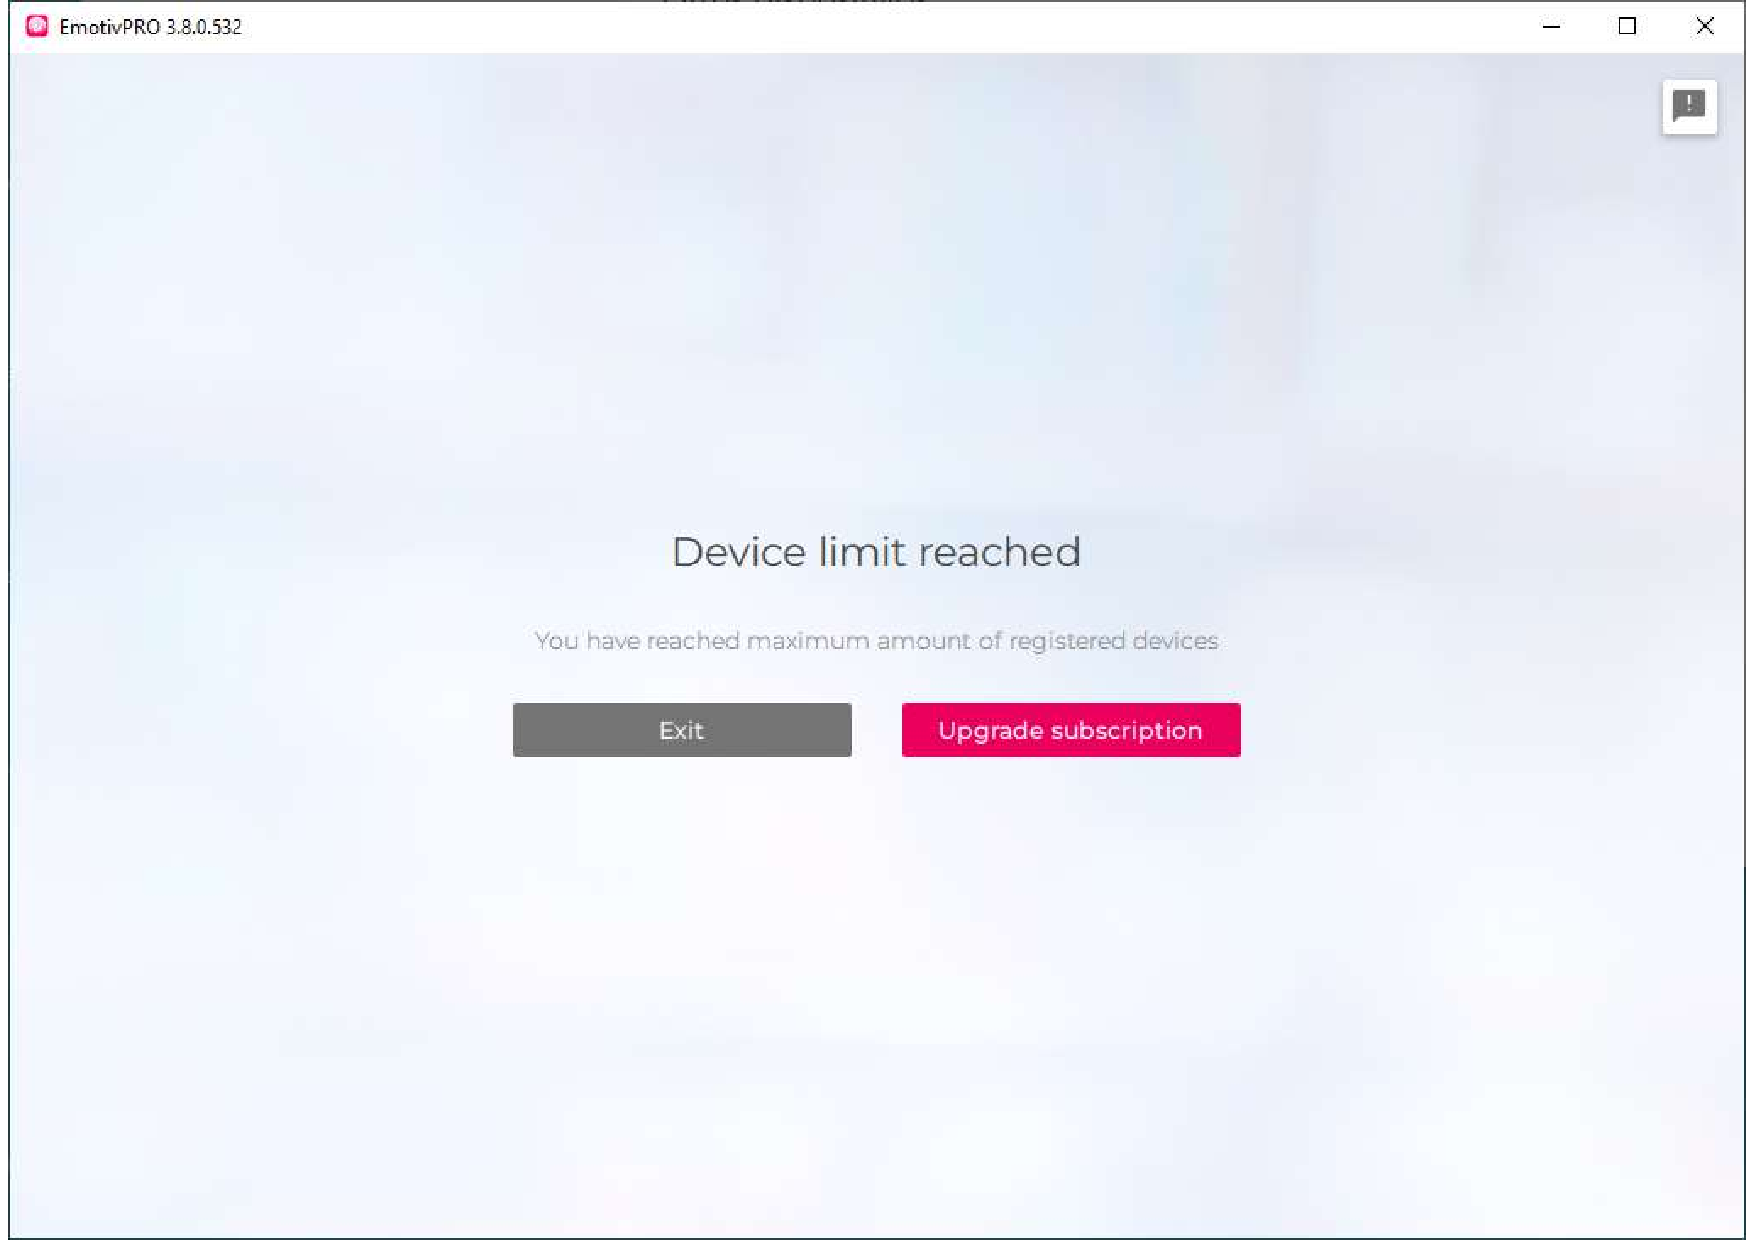
\includegraphics[width=0.4\textwidth]{img/LimiteDispositivosEmotiv.pdf}
    \caption{Aviso de límite de dispositivos alcanzado.}
    \label{fig: LimiteDispositivos}
\end{figure}

Por lo tanto, tras la acumulación de varias horas de pruebas e investigación, se comprueba la hipótesis de que la licencia y la primera conexión limitan el uso del dispositivo a un solo ordenador. Otra conclusión que se puede sacar de ello es que su uso para terapia queda limitado, ya que el dispositivo está destinado a ser empleado en un único ordenador con un único usuario que posea las licencias adecuadas; cabiendo la posibilidad de mejorar las licencias, lo que implica pagar más dinero.

\subsection{Problema conexión MN8.}
Durante el proceso de conexión del dispositivo MN8 con el ordenador, se experimentó un problema técnico. El dispositivo MN8 se conectaba correctamente al ordenador, pero dentro de la configuración y posicionamiento del dispositivo, la calidad de la señal era del 0\%. Esto implicaba que, a pesar de que el dispositivo era detectado, no había una comunicación efectiva entre el dispositivo y el ordenador.

Para resolver este problema, se realizó un cambio de sensores por los que tienen 3 filamentos, lo que aumentó la superficie de contacto. Este cambio permitió finalmente una calidad de conexión óptima del 100\%.

Tras el cambio de sensores, se obtuvo una correcta solución al problema. La calidad de la conexión entre el dispositivo MN8 y el ordenador mejoró significativamente, pasando de un 0\% a un 100\%. Esto permitió una comunicación efectiva entre el dispositivo y el ordenador, facilitando así la realización de las tareas necesarias. Por lo tanto, se concluye que el cambio de sensores fue una solución efectiva para el problema experimentado.

\subsection{Problema con PsychoPy Coder.}
El experimento fue inicialmente diseñado con PsychoPy Coder, que es un entorno de programación con código para la realización de experimentos que permite el uso de dispositivos de Emotiv para la lectura de EEG. En este entorno se generaba un error en la conexión con el dispositivo Emotiv que no permitía ni la lectura de EEG ni la correcta ejecución del experimento. A partir de este problema se decidieron probar las mismas rutinas diseñadas en PsychoPy Builder, que es el entorno de programación por bloques de PsychoPy. De esta manera no se obtienen errores en la ejecución y pueden visualizarse sin problema todas las rutinas del experimento y añadir el componente de\textit{ Emotiv Recording}.

\capitulo{7}{Lineas de trabajo futuras}


Este capítulo debería ser informe crítico indicando cómo se puede mejorar el proyecto, o cómo se puede continuar trabajando en la línea del proyecto realizado.



\bibliographystyle{apalike}
\bibliography{bibliografia}

\end{document}
